\documentclass[oneside]{amsart}
\usepackage[left=1.25in,right=1.25in,top=0.75in,bottom=0.75in]{geometry}
\usepackage{graphicx}
\linespread{1.05}
\usepackage{mathpazo}
\usepackage{amsfonts,amssymb,latexsym,amsmath, amsthm}
\usepackage{tikz-cd}
\usepackage{comment}
\usepackage{mathrsfs}
\usepackage{stmaryrd}
\usepackage{tcolorbox} 
\usepackage{hyperref}
\usepackage{newpxmath}
\usepackage{eulervm}
\hypersetup{
    colorlinks = true,
    linkbordercolor = {red}
}
\theoremstyle{definition}
%% this allows for theorems which are not automatically numbered
\newtheorem{defi}{Definition}[section]
\newtheorem{theorem}{Theorem}[section]
\newtheorem{lemma}{Lemma}[section]
\newtheorem{obs}{Observation}
\newtheorem{exercise}{Exercise}[section]
\newcommand{\heg}{\text{Heg}}
\newtheorem{rem}{Remark}[section]
\newtheorem{construction}{Construction}[section]
\newtheorem{prop}{Proposition}[section]
\newtheorem{coro}{Corollary}[section]
\newtheorem{disc}{Discussion}[section]
\DeclareMathOperator{\spec}{Spec}
\DeclareMathOperator{\Lim}{Lim}
\DeclareMathOperator{\im}{im}
\DeclareMathOperator{\obj}{obj}
\DeclareMathOperator{\ext}{Ext}
\DeclareMathOperator{\Int}{Int}
\DeclareMathOperator{\tor}{Tor}
\DeclareMathOperator{\ann}{ann}
\DeclareMathOperator{\id}{id}
\DeclareMathOperator{\proj}{Proj}
\DeclareMathOperator{\gal}{Gal}
\DeclareMathOperator{\coker}{coker}
\newcommand{\degg}{\textup{deg}}
\newtheorem{ex}{Example}[section]
%% The above lines are for formatting.  In general, you will not want to change these.
%%Commands to make life easier
\newcommand{\RR}{\mathbf R}
\newcommand{\aff}{\mathbf A}
\newcommand{\ff}{\mathbf F}
\usepackage{mathtools}
\newcommand{\cccC}{\mathbf C}
\newcommand{\oo}{\mathcal{O}}
% \newcommand{\ZZ}{\mathbf Z}
\newcommand{\pring}{k[x_1, \ldots , x_n]}
\newcommand{\polyring}{[x_1, \ldots , x_n]}
\newcommand{\poly}{\sum_{\alpha} a_{\alpha} x^{\alpha}} 
\newcommand{\ZZn}[1]{\ZZ/{#1}\ZZ}
% \newcommand{\QQ}{\mathbf Q}
\newcommand{\rr}{\mathbb R}
\newcommand{\cc}{\mathbf C}
\newcommand{\complex}{\mathbf {C}_\bullet}
\newcommand{\nn}{\mathbb N}
\newcommand{\zz}{\mathbb Z}
\newcommand{\PP}{\mathbb P}
\newcommand{\cat}{\mathbb {C}}
\newcommand{\ca}{\mathbf}
\newcommand{\zzn}[1]{\zz/{#1}\zz}
\newcommand{\qq}{\mathbb Q}
\newcommand{\calM}{\mathcal M}
\newcommand{\latex}{\LaTeX}
\newcommand{\V}{\mathbf V}
\newcommand{\tex}{\TeX}
\newcommand{\sm}{\setminus} 
\newcommand{\dom}{\text{Dom}}
\newcommand{\lcm}{\text{lcm}}
\DeclareMathOperator{\GL}{GL}
\DeclareMathOperator{\Hom}{Hom}
\DeclareMathOperator{\aut}{Aut}
\DeclareMathOperator{\SL}{SL}
\DeclareMathOperator{\inn}{Inn}
\DeclareMathOperator{\card}{card}
\newcommand{\sym}{\text{Sym}}
\newcommand{\ord}{\text{ord}}
\newcommand{\ran}{\text{Ran}}
\newcommand{\pp}{\prime}
\newcommand{\lra}{\longrightarrow} 
\newcommand{\lmt}{\longmapsto} 
\newcommand{\xlra}{\xlongrightarrow} 
\newcommand{\gap}{\; \; \;}
\newcommand{\Mod}[1]{\ (\mathrm{mod}\ #1)}
\newcommand{\p}{\mathfrak{p}} 
\newcommand{\rmod}{\textit{R}-\textbf{Mod}}
\newcommand{\idealP}{\mathfrak{P}}
\newcommand{\ideala}{\mathfrak{a}}
\newcommand{\idealb}{\mathfrak{b}}
\newcommand{\idealA}{\mathfrak{A}}
\newcommand{\idealB}{\mathfrak{B}}
\newcommand{\X}{\mathfrak{X}}
\newcommand{\idealF}{\mathfrak{F}}
\newcommand{\idealm}{\mathfrak{m}}
\newcommand{\s}{\mathcal{S}}
\newcommand{\cha}{\text{char}}
\newcommand{\ccc}{\mathfrak{C}}
\newcommand{\idealM}{\mathfrak{M}}
\usetikzlibrary{decorations.pathmorphing} 
\newcommand{\overbar}[1]{\mkern 1.5mu\overline{\mkern-1.5mu#1\mkern-1.5mu}\mkern 1.5mu}

%Itemize gap:

% \pagecolor{black}
% \color{white}
% Author info
\begin{document}
\title{Math 425A Notes}
\author{Juan Serratos}
\email{jserrato@usc.edu}
\date{ September 17, 2022 \\ {Department of Mathematics, University of Southern California}}
\address{Department of Mathematics, University of Southern California, 
Los Angeles, CA 90007}
\maketitle
\setcounter{tocdepth}{4}
\setcounter{secnumdepth}{4}
\tableofcontents
\begin{comment}
\section{Lecture Date: Unknown, Chapter 1. $\S 4$} 
\subsection{$\S 4.1$: Notation and Definitions} The usual notion of cardinality is easy to comprehend if we use our intuition to generalize examples; for example, if we have the set $\{ 1, 2, 3 \}$, we define the cardinality of the set to be the \textit{number of elements} in this set, and so $\card\{1,2, 3 \} = 3$. However, our intuition cannot readily comprehend sets where ambiguity (and easy confusion) occurs: consider the set of all rational numbers $\qq$ and the set of all natural numbers $\nn := \nn_{>0}$; how can you compare the cardinalities of these sets? You know that $\nn \subseteq \qq$, and so intuitively we think of $\qq$ as being `bigger' than $\nn$, yet we would, perhaps naively, state that their cardinalities are the same as the sets are both infinitely big. This notion of cardinality, rather than thinking about \textit{counting} as we do in everyday life, can be better described by function relations: specifically hinging on the definitions of injective $\&$ surjective functions. Coming back to our example of $\nn$ and $\qq$, we know that $\nn \subseteq \qq$ so we can apply the canonical injection to $\nn$, i.e. $i \colon \nn \to \qq$, where $i(n) = n$ for all $n \in \nn$. As we have this total embedding of $\nn$ into $\qq$, via our injection, we will write $\card \nn \leq \card \qq$.
\begin{defi}
Let $A$ and $B$ be nonempty sets. We abuse the following notation:
\begin{itemize}
	\item[(i)] $\card A \leq B$ if there exists an injective function $f \colon A \to B$;
	\item[(ii)] $\card A \geq \card B$ if there exists a surjective function $g \colon A \to B$;
	\item[(ii)] $\card A = \card B$ if there exists an injective and surjective (i.e. bijective) function $h \colon A \to B$.
\end{itemize}	
\end{defi}
\begin{theorem}
	Let $A$ and $B$ be sets.
	\begin{itemize}
		\item [(a)] If $A \subseteq B$, then $\card A \leq \card B$.
		\item [(b)] If $\card A \leq \card B$ and $\card B \leq \card C$, then $\card A \leq \card C$.
		\item [(c)] $\card A \leq \card B$ if and only if $\card B \geq \card A$.
		\item [(d)] Either $\card A \leq \card B$ or $\card B \leq \card A$ holds true.
		\item [(e)] (Schroder-Bernstein) If $\card A \leq \card B$ and $\card B \leq \card A$, then $\card A = \card B$.
	\end{itemize}
\end{theorem}
\begin{proof}(a) If $A \subseteq B$, then we can apply the canonical injection $i \colon A \to B$, which is of course an injective function. Thus $\card \leq \card B$. (b) Suppose that $\card A \leq \card B$ and $\card B \leq \card C$, i.e. we have injective functions $f \colon A \to B$ and $g \colon B \to C$. Then consider $g\circ f \colon A \to C$; we have to show this is injective. Suppose that $g \circ f (x_1) = g \circ f(x_2)$, then $g(f(x_1)) = g(f(x_2))$ gives us that $f(x_1) = f(x_2$ as $g$ is injective and $x_1 = x_2$ as $f$ is injective. Hence we have an injective function from $A$ to $C$, i.e. $\card A \leq \card C$. (c) Suppose that $f \colon A \to B$ is injective. Then $f$ has a left inverse, say, $h \colon B \to A$, and so $h \circ f = 1_A$. But we may also look at this statement as saying that $h$ has a right inverse, $f$, and so $h$ is surjective. Thus $h \colon B \to A$ is surjective, and the corresponding cardinality rephrasing is true. The other direction follows by a similar argument. $(d)$ $\&$ $(e)$ Omitted.
\end{proof}
As a shorthand, we will often write $A \sim B$ to mean that $\card A = \card B$. As the notation suggests, this relation is indeed an equivalence relation, i.e. the relation is reflexive, symmetric, and transitive. That is, $A \sim A$ since $\id \colon A \to A$ is a bijection on itself; if $A \sim B$, then $h \colon A \to B$ is a bijection, which implies that there is an inverse bijection $h^{-1} \colon B \to A$, and thus $B \sim A$; the transitivity property follows the same form as these two arguments, and is easy to show given the fact that the composition of two bijective functions is itself bijective. 
\subsection{$\S 4.2$: Generating Equivalences}
\begin{lemma}
	Assume $A \cap B = X \cap Y = \varnothing$. Let $f \colon A \to X$ and $g \colon B \to Y$ be bijection, and define a function $h \colon A \cup B \to X \cup Y$ by the following rule 
	\[
	h(c) = \begin{cases}
		f(c) & \text{if }c \in A  \\ 
		g(c) & \text{if } c \in B.
	\end{cases}
	\] Then $h$ is bijection.
\end{lemma}
\begin{proof}
	As $f$ and $g$ are bijections themselves, then they have corresponding unique inverses $f^{-1}$ and $g^{-1}$, respectively. We define the function $\ell \colon X \cup Y \to A \cup B$ to be the piecewise function given by $c \mapsto f^{-1}(c)$ if $c \in X$ and $c \mapsto g^{-1}(c)$ if $c \in Y$. To show that we have the bijection between the two sets we show that $\ell$ is a two-sided inverse of $h$. So, if $c \in X$, then $h \circ \ell (c) = h(\ell (c)) = h(f^{-1}(c)) = f(f^{-1}(c)) = c$, and if $c \in Y$, initially, then $h \circ \ell (c) = h(\ell (c)) = h (g^{-1}(c)) = g(g^{-1}(c)) = c$. Checking that $\ell$ is also a left inverse is easy from seeing after this. 
\end{proof}
\begin{coro} Let $A,B, X,$ and $Y$ be sets. If $A \cap B = X \cap Y = \varnothing$,  $A \sim X$, and $B \sim Y$, then $A \cup B \sim X \cup Y$.
\end{coro}
\begin{exercise}[4.1.]
	Assume that $\card A \leq \card X$ and $\card B \leq \card Y$. Prove that $\card (B^A) \leq \card (Y^X)$. Hint: Consider a function $\Phi \colon B^A \to Y^X$ of the form $\Phi (f) = h \circ f \circ k$, where $k \colon X \to A$ and $h \colon B \to Y$ are certain functions. Theorem [3.8] [Slogan: `Left inverse if and only if injective; right inverse if and only if surjective'].
\end{exercise}
\begin{proof}
	(Side note: the notation used to denote the set of functions is awful, and we will prefer the category theory option; that is, $B^A := \Hom _{\mathbf{Sets}} (A, B)$ denotes the set of functions from $A$ to $B$. Thus we want to show that $\card ( \Hom (A,B) ) \leq  \card (\Hom (Y,X))$. ) By hypothesis, we have that there are injective functions $f \colon A \to X$ and $g \colon B \to Y$. Now there are also corresponding left inverses for these functions, say, $k \colon X \to A$ and $h \colon Y \to B$, respectively. We will construct the function $\Phi \colon \Hom (A, B) \to \Hom (Y,X)$, by mapping every $\varphi \in \Hom (A,B)$ to $ h \circ \varphi \circ k \colon X\to Y$, which is indeed a function in $\Hom (Y,X)$. We must show that $\Phi$ is injective. Consider $\Phi (f_1) = \Phi (f_2)$. Then, we will begin the process of inverting: 
	\begin{align*}	
		\Phi (f_1) &= \Phi (f_2) \\
		h \circ f_1 \circ k &= h \circ f_2 \circ k \\
		g \circ h \circ  f_1 \circ k &= g \circ h \circ f_2 \circ k \\
		f_1 \circ k &=  f_2 \circ k \\
		f_1 \circ k \circ f &= f_1 \circ k \circ f \\ 
		f_1 & = f_2
	\end{align*}
	Therefore the function as constructed is indeed an injection, and it follows that $\card \Hom (A, B) \leq \card (\Hom (X, Y))$.
\end{proof}
\begin{prop}
For any set $A$, $\card A < \card \mathcal P (A)$.	
\end{prop}
\begin{proof}
	We want to show that there is a strict injection from $A$ to $\mathcal P(A)$; that is, there is an injection $A \to \mathcal P(A)$, but not a surjection. Firstly, we construct a function $\varphi \colon A \to \mathcal P(A)$ by mapping every $x \in A$ to $\{x \} \in \mathcal P(A)$. Clearly this function is injective since if $\varphi(x_1) = \varphi(x_2)$ then $\{x_1 \} = \{x_2 \}$, and so $x_1 = x_2$. To show that there doesn't exist a surjection is a bit more tedious. Let $g \colon A \to \mathcal P(A)$ be any function mapping. Define $B := \{x \in A \colon x \notin g (x) \}$. We claim that $B \notin \im (g)$, i.e. $g(x) \neq B$ for any $x \in A$ ($x$ under the map $g$ doesn't generate the set $B$). By contradiction, suppose that $g(x) = B$ for some $a \in A$. Then then $x \notin B$, as $x \in A$ and $x \in g(x)$. On the other hand, if $x \notin B = g(x)$, then $x \in B$ by definition of $B$. Hence the claim follows. 
\end{proof}
\begin{exercise}[4.2.] Prove that for any set $A$, we have that $\mathcal P (A) \sim \Hom (A, \{0,1 \})$.
\end{exercise}
\begin{proof}
	We define a function $\Omega \colon \mathcal P (A) \to \Hom(A, \{ 0,1 \} )$ as follows. If $B \subseteq A$, we let $\Omega (B) \colon \mathcal P (A) \to \Hom (A, \{0,1 \})$ by the rule 
	\[
	\Omega (B) (a) = \begin{cases}
		1, & \text{if } a \in B \\
		0, & \text{if } a \notin B.
	\end{cases}
	\] On the other hand, we define the function $\Psi \colon \Hom (A, \{0,1 \}) \to \mathcal P(A)$ by the rule $\Psi (f) = f^{-1}(1) := f^{-1} (\{1\})$. As the construction hints, these two functions are indeed inverses of one another:
	\[
	\Omega (\Psi(f))(a) = \begin{cases}
		1, & \text{if } a \in f^{-1} (1) \\
		0, & \text{if } a \notin f^{-1} (1) 
	\end{cases} = \begin{cases}
		1, & \text{if } a = f(1) \\
		0, & \text{if } a \neq  f(1) 
	\end{cases} = f(a), \forall a \in A
	\] Thus we have $\Omega \circ \Phi (f) = f$ for all $f \in \Hom (A, \{0,1 \})$. Similarly to checking this side of inversion, $\Psi(\Omega(B)) = \Omega (B)^{-1} (1) = B$, for all $B \in \mathcal P (A)$.
\end{proof}
\subsection{$\S 4.3:$ Finite and Infinite Sets.} For each $n \in \nn$, let $J_n := \{1, \ldots, n \}$. It can be shown, but will be omitted, that for $m, n \in \zz$, one has $\card J_m \leq \card J_n$ if and only if $m \leq n$. Thus it makes sense to say that $\card J_n = n$ for all $n \in \nn$. We also define $\card \varnothing = 0$
\begin{defi}
A set is called \textbf{finite}	if $\card A = \card J_n$ for some $n \in \nn$, or if $A = \varnothing$. A set is called \textbf{infinite} if it is not finite.
\end{defi}
\begin{prop}
If $A$ and $B$ are finite, disjoint sets, then $\card (A\cup B)$ is finite, and $\card (A\cup B) = \card A + \card B$.	
\end{prop}
\begin{proof}
	Since $A$ and $B$ are finite, there exists integers $m$ and $n$ such that $A \sim J_m$ and $B \sim J_n \sim \{m+1, m+2, \ldots, m+n \}$. Since $A \cap B$ and $J_m \cap \{m+1, m+2, \ldots, m +n \}$ are empty, then Lemma 1.1 gives us that $\card (A \cup B) \sim J_m \cup \{m+1, m+2, \ldots, m+n \} = J_{m+n}$, i.e. $\card (A\cup B) = m+n = \card A + \card B$. 
\end{proof}
However, if we simply have that $A$ and $B$ are any finite sets (not necessarily disjoint), then $A \cup B$ is finite since we can always make create a disjoint as we can write $A \cup B = A \setminus B \cup B $, which are disjoint, and so the claim follows with applying the preceding proposition.

\begin{prop}
Let $A$ and $B$ be finite sets. Then $ \card (\Hom (B, A)) = \card (A)^{\card (B) }$, and $\card (\mathcal P (A)) = 2^{\card A }$. 
\end{prop}
\begin{proof}
	As both $A$ and $B$ are finite sets, then there are some $m, n \in \nn$ such that $A \sim J_m$ and $B \sim J_n$. By Exercise 4.1., it follows that $\Hom (B,A) \sim \{1, \ldots, m\}^n$, i.e. the set of $n$-tuples whose entries are $X = \{1, \ldots, m \}$. Since there are $m$ choices for the $n$ entries, then there are $m^n = \card A ^{\card B}$ elements in this set. 
	
	For the second part of the statement, we use Exercise $4.1.$ As $\mathcal P(A) \sim \Hom (A, \{0,1 \})$, then \\ $\card \mathcal P (A) = \card (\Hom (A, \{0,1 \}) = \card \{0,1 \}^{\card A } = 2^{\card A }$.
\end{proof}
We should note here that although we've been using things from the natural numbers, the set of natural numbers, $\nn$, isn't itself finite... this shouldn't be too surprising. There's many ways to show this fact, but we'll give a simple argument: Suppose that $\nn$ is finite, then there is some $J_n$ such that $\nn \sim J_n$. And so we have a surjection $f \colon J_n \to \nn$. Yet we can easily construct a surjection $g \colon \nn \to J_{n+1}$ where $g(j) = j$ for $j \in J_{n+1}$ and $g(j) = 1$ for $j >n+1$. But then $g \circ f \colon J_n \to J_{n+1}$ must also be a surjection as the composition of surjective maps is itself surjective, but this is a contradiction as this would imply $\card J_n = n \geq \card J_{n+1} = n +1$. Thus $\nn$ cannot be finite. However, we will treat $\nn$ as being our smallest infinite set. 
\begin{defi}
Let $A$ be set. We say that $A$ is \textbf{countable} if $\card A \leq \card \nn$. We say $A$ is \textbf{countably infinite} if $\card A = \card \nn$. We say that $A$ is uncountable if it is not countable. 	
\end{defi}

An often useful equivalent notion of `countable' cardinality of some set $A$ is if it can be indexed by $\nn$; that is to say that there exists a sequence $(a_j)_{j=1}^\infty$ whose image $\{a_j \}_{j=1}^\infty$ is equal to $A$. We say that $(a_j)_{j=1}^\infty$ is an \textbf{enumeration} of the elements in $A$, as we can write all the elements to appear in the `list' $(a_1, a_2, a_3, \ldots)$. 
\begin{prop}
Let $A$ be an infinite set. Then $A$ contains a countably infinite subset. 	
\end{prop}
\begin{coro}
A set $A$ is infinite if and only if $\card A \geq \card \nn$.	
\end{coro}
\begin{proof}
	If $A$ is infinite, then it has a countably infinite subset, say, $B$. Then $B = \card \nn$, and as $B \subseteq A$, then $\card B \leq \card A$, so $\card \nn \leq \card A$. Now suppose that $\card A \geq \card \nn$. Then as $\card \nn > \card J_m$ for some $m \in \nn$, then $\card A > \card J_m$, i.e. not finite, and so $A$ is infinite. 
\end{proof}
\begin{theorem}
A set $A$ is infinite if and only if there exists a proper subset $B$ of $A$ such that $A \sim B$.
\end{theorem}
\begin{exercise}[4.3.] Let $A$ and $B$ be sets, and assume $f \colon A \to B$ and $g \colon B \to A$ are injective functions.
\begin{itemize}
	\item [(a)] Assume additionally that $A$ is finite. Prove that $f$ and $g$ must also be bijections.
	\item [(b)] Show by way of an example that both $f$ and $g$ may fail to be bijective if we do not assume that $A$ is finite. 
\end{itemize}
\end{exercise}
\begin{proof}
	(a) As $f$ and $g$ are injections, then $\card A \leq \card B$ and $\card B \leq \card A$, and so $\card A = \card B$, by Schorder-Berstein. But as $A$ is finite then $\card A = \card J_m$ for some $m \in \nn$, and so $B$ is itself finite. Consider $f(A) = \{f(a) \colon a \in A \} \subseteq B$. As $A$ is finite, then we can also enumerate it as $\{a_1, \ldots, a_n \}$, and as $f$ is injective then all outputs in $B$ have distinct inputs coming from $B$, and so $ \card ( \{f(a_1), \ldots, f(a_n) \}) =\card (f(A)) = n$. So the cardinality of the image of $A$ under $f$ is itself the cardinality of the codomain $B$; thus we must have that $f(A) = B$. Therefore $f$ is a bijection. We can apply nearly the exact same argument for $g \colon B \to A$ to find that $g(B) = A$, and we have the other bijection. 
	
	(b)
\end{proof}
\begin{exercise}
	Let $A$ and $B$ be finite sets. Assume that $A$ is infinite, $B$ is countable, and $A$ and $B$ are disjoint. Prove that $A \sim A \cup B$. Hint the strategy of Theorem [1.2.]. may be useful. You may also use the fact that the union of two countable sets is countable.  
\end{exercise}
\begin{proof}
	As $A \subseteq A \cup B$, then we have an injection from $f \colon A \to A\cup B$, namely the canonical injection. Now we must find another injection from $A \cup B \to A$. As $B$ is countable, we can enumerate it by, say, $B = \{b_0, b_1, \ldots \}$, and as $A$ is infinite then it contains a countably infinite subset, say $T= \{a_0, a _1, \ldots \} \subseteq A$. We define a map $\varphi \colon A \cup B \to A$, where 
	\[
	\varphi (a) = \begin{cases} a & \text{if } a \in A\setminus (T \cup B) \\
	a_{2n+1} & \text{if } a = b_n \text{ for } b_n \in B \\
	a_{2n} & \text{if } a= a_n \in T\setminus B 
	\end{cases}
	\] This does indeed produce a well-defined injective function from $A \cup B \to A$. Thus by Schroder-Berstein, we have that there is some bijection from $A \to A \cup B$, i.e. $A \sim A \cup B$. 
\end{proof}
\begin{exercise} Let $X$ and $Y$ be sets. Assume that $Y$ is countable and $X \setminus Y$ is infinite. Prove that $X \sim X \cup Y \sim X \setminus Y$. Hint: Each of the equivalences can be done extremely quickly if you use the previous exercise and some set manipulations.
\end{exercise}
\begin{proof}
	By the previous exercise, as $Y$ is countable and $X \setminus Y$ is infinite, and clearly $(X\setminus Y) \cap Y = \varnothing$, then we have that $X \setminus Y \sim (X \setminus Y) \cup Y=X \cup Y$; hence $X \setminus Y \sim X \cup Y$. It remains to show that $X$ has the same cardinality as one of these. Trivially, we have that $X \setminus Y \subseteq X$, since if we take $x \in X \setminus Y$ then $x \in X$ and $x \notin Y$, and so $x \in X$, vacuously. Now $X \subseteq X \cup Y$ as well. So then $ \card (X \setminus Y ) \leq \card X$ and $\card X \leq \card (X\cup Y)$. Thus $\card(X\setminus Y) \leq \card X \leq \card (X \cup Y)$. But as $\card (X\setminus Y) = \card (X\cup Y)$, then we must have that $X \sim X \setminus Y \sim X \cup Y$.
\end{proof}
\subsection{$S4.4:$ Countable Sets}
\begin{prop}
$\nn \times \nn$ is countably infinite.	
\end{prop}
\begin{proof}
	The function $f \colon \nn \times \nn \to \nn$ defined by $f((m,n))=2^n \cdot 3^m$ is injective. Let $f((m,n)) = f((x,y))$. Then $2^n \cdot 3^m = 2^x \cdot 2^y$, which implies that $n=x$ and $m=y$ by the uniqueness of primes. Thus we have $\card (\nn \times \nn) \leq \card \nn$. On the other hand, we let $g \colon \nn \to \nn \times \nn $ where $g (n) = (n,0)$. This is injective since if $g(n)=g(m)$ for some $n, m \in \nn$, then $(n,0) = (m, 0)$; thus we must have that $n=m$. Hence $g$ is injective and $\card \nn \leq \card (\nn \times \nn)$. Thus $\card \nn = \card \nn \times \nn$ and $\nn \times \nn$ is countably infinite. 
\end{proof}
If $\mathcal A$ is a countable collection of sets, then we say that $\bigcup _{A \in \mathcal A} A$ is a \textit{countable union}. If $\mathcal A$ is finite, we call it a \textit{finite union}. Using this terminology, the following statement's slogan is that the countable union of countable sets is countable.
\begin{prop}
Let $\{A_j\}_{j=1}^\infty$ be a countable collection of countable sets. Then the union $$S = \bigcup_{j=1}^\infty A_j$$ is also countable. 	
\end{prop}
\begin{proof}
	We define a function $f \colon \nn \times \nn \to S$ as follows. For each $j \in \nn$, let $g_j \colon \nn \to A_j$ be a (the correspond) surjection. Define $((j,k)) = g_j(k)$ for each $(j,k) \in \nn \times \nn$. Then $f$ we claim that $f$ is surjective. If we take some $x \in S$, then $x \in A_j$ for some $j \in \nn$ in the countable collection of countable sets $\{A_i\}_{i=1}^\infty$. But as $g_j$ is itself surjective, then we have $x=g_j(k)=f(j,k)$ for some $k \in \nn$. It follows that $\card S \leq \card (\nn \times \nn ) = \card \nn$. That is to say, $S$ is countable. 
\end{proof}
This proposition has actually some important things to say about the usual sets we work with. As we can write $\zz = \nn \cup -\nn \cup \{0 \}$, where $-\nn$ denotes the set $\{-n \}_{j=1}^\infty$, then $\zz$ is itself countable. Similarly, $\qq$ is countable since the function $\varphi \colon \zz \times (\zz\setminus \{0\}) \to \qq$ defined by $\varphi ((a,b)) = \frac{a}{b}$ is a surjection. 
\begin{exercise}
	Let $X$ be a countable set.
	\begin{itemize}
		\item [(a)] Prove that $X^{n+1} \sim X^n \times X$ for any $n \in \nn$. (This not difficult, be careful with the notation.)
		\item [(b)] Prove inductively that $X^n$ is countable for any $n \in \nn$.
	\end{itemize}
\end{exercise}
\begin{proof}
	(a) For $n=1$, then $X^2 \sim X^1 \times X$ is clear since $X^1 \times X = X^2$, and so just take the identity map on $X^2 \to X^2$. We define a map $f\colon X^{n+1} \to X^n \times X$ by letting $f( (x_1, \ldots, x_{n+1}))= ((x_1, \ldots, x_n), x_{n+1})$, and another map $g \colon X^n \times X \to X^{n+1}$ by defining $g((x_1\ldots, x_n), x_{n+1`})$; note that the indexing works as each $X$ is countable. These functions can be easily realized to be inverses of each other, and so we have bijections $f$ and $g$. Thus $X^{n+1} \times X^n \times X$ for each $n \in \nn$.
	
	(b) For the case of $n=1$, we have that $X^1 = X$, which is countable by hypothesis. Now assume that $X^k$ is countable for $k \in \nn$ and $k \geq 1$. We will consider $X^{k+1}$. Then, from the first part, we know that $X^{k+1} \sim X^k \times X$. We know that $X$ and $X^k$ are countable sets, once again by hypothesis; thus we have injective maps $f \colon X^k \to \nn$ and $g \colon X \to \nn$. We define the map $\psi \colon X^k \times X \to \nn \times \nn$ by $\psi ((x,y)) = (f(x), g(y))$; the claim is that this map is an injection. Suppose that $\psi ((x,y)) = \psi ((z,w))$ for $(x,y)$ and $(z,w)$ in $X^k \times X$. Then $(f(x), g(y)) = (f(z), g(w))$, and so we must have that $f(x) = f(z)$ and $g(y) = g(w)$, but as $f$ and $g$ are both injective we get that $x=z$ and $y=w$. Hence the claim is true and $\psi$ is indeed an injection. Thus $\card (X^k \times X) \leq \nn \times \nn = \card \nn$ (as $\nn \times \nn$ is countably infinite). By the initial part, we have that $X^{k+1} \sim X^k \times X$, and therefore $\card(X^{k+1}) \leq \card\nn$, i.e. $X^{k+1}$ is countable. 
\end{proof}
\subsection{$\S 4.5:$ Uncountable Sets}
\begin{prop}
If $X$ is any set that contains at least two elements and $J$ is countably infinite, then $\Hom (J,X)$ is uncountable. In particular, $\Hom (\nn , \{0,1 \})$ is uncountable. 	
\end{prop}
\begin{proof}
	Since $\card X \geq \card ( \{0,1 \} )$, and $\card (J) \geq \card \nn$, we have 
	\begin{align*}
		\card (\Hom (J,X)) &\geq \card(\Hom (\nn, \{0,1 \} )) \; \; \; \; \; \; \; [Exercise\;  4.1.] \\
		&= \card \mathcal P (\nn) \; \; \; \; \; \; \; \;[Exercise\;  4.2.]  \\
		&> \card \nn \; \; \; \; \; \; \; \; \; \; \; \; \;[Proposition \; 1.1.]
	\end{align*}
\end{proof}
\section{Lecture Date: Sept. 19, Chapter 2. $\S 2 - 2.3$}
\subsection*{$\S: ``2.0"$} 
\begin{defi} Let $X$ be a set. A \textbf{metric} on $X$ is a function $d \colon X \times X \to \rr$, satisfying the following properties:
\begin{itemize}
	\item [(i)] (Nonnegativity) $d(x,y) \geq 0 $ for all $x,y \in X$, with $d(x,y) = 0$ if and only if $x=y$. 
	\item [(ii)] (Symmetry) $d(x,y) = d(y,x)$ for all $x,y \in X$. 
	\item [(ii)] (Triangle Inequality) $d(x,y) \leq d(x,z) + d(z,y)$ for all $x, y, \in X$. 
\end{itemize}
The pair $(X,d)$ is called a metric space, and, if context is understood with the metric, then we will typically just say that $X$ is a metric space. Elements of the set $X$ are just called \textit{points}. The (real) number $d(x,y)$ is called the \textit{distance} from $x$ to $y$, and a metric is sometimes called a \textit{distance function}. 
\end{defi}
Our intuition for this concept likely comes from our experience of using the real line to simulate notions of distance between real numbers where we consider the distance between points on the real line from their distance from $0$, i.e. we do this with the absolute value \textit{metric}, $| \cdot | \colon \rr \to \rr_{\geq 0}$, where, for any $x \in X$, 
\[
|x| = \begin{cases}
	x & \text{if $x \geq 0$} \\
	-x & \text{if $x < 0$}
\end{cases}
\]
\begin{ex} On a vector space $V$, $d \colon V \times V \to \rr$, where $(x,y) \mapsto d(x,y) := \|x-y\|$ is a metric. Recall that this is a \textit{norm} on $V$ which satisfies $\|v \| \geq 0$, and $\|v \| =0$ if and only if $v$ is the zero vector in $V$, $\|\alpha v \| = |\alpha | \|v \|$ for any scalar $\alpha$ and any $v \in V$, and $\|u+v \| \leq \|u \| + \| v \|$ whenever $u,v \in V$.

Another example is the discrete case where we let $X$ be any set and set $d(x,y) = 0$ if $x = y$ and $d(x,y) = 1$ if $x \neq y$. We call this the discrete metric. 
\end{ex}


\subsection{$\S2.1.$ Open Balls in a Metric Space}

Suppose that we fix some point $P$ is a metric space $(X, d)$. It is often useful to talk about points in the metric space that are \textit{close} to $P$. We encapsulate this notion into the definition of the (open) ball of radius $r$ centered at $P$ in $X$, that is, $$B_{(X,d) } (P, r) = \{ s \in X \colon d(P,s) < r \}.$$ If the notation for our given metric space is clear, then we will often write $B_X(P,r)$, $B_d (P, r)$, or simply just $B(P, r)$. 

Now, we want to talk about \textit{submetrics}, which are simple to talk about since if we're given a metric space $(X,d)$ such that $Y \subseteq X$, then $(Y,d)$ is itself a metric since we're just restricting $X$ to a (possibly) smaller (or equivalent) size to itself. Moreover, if $P \in Y$ is 'near the edge' of $Y$, then $B_Y(P, r)$ can be possibly be smaller than $B_X(P,r)$. Indeed,  $B_Y (P, r) = \{s \in X \colon d(P,s) < r \} = \{s \in X \colon d(P, s) < r \} \cap Y = B_X(P,r) \cap Y.$

\subsection{$\S2.2.$ Interior Points}
\begin{defi}
Let $(X,d)$ be a metric space and let $U$ be a subset of $X$. A point $P \in U$ is called an \textbf{interior point} of $U$ with respect to $X$ if there exists some $r >0$ such that $B_X (P, r) \subseteq U$. The set of all such interior points of $U$ with respect to $X$ is called the \textbf{interior} of $U$ with respect to $X$, and we will denote it by $\Int _X(U)$, i.e. $\Int_X(U) = \{ x \in U \colon \text{$x$ is an interior point of $U$ with respect to $X$} \}$. 	
\\
\begin{figure*}[h!] 
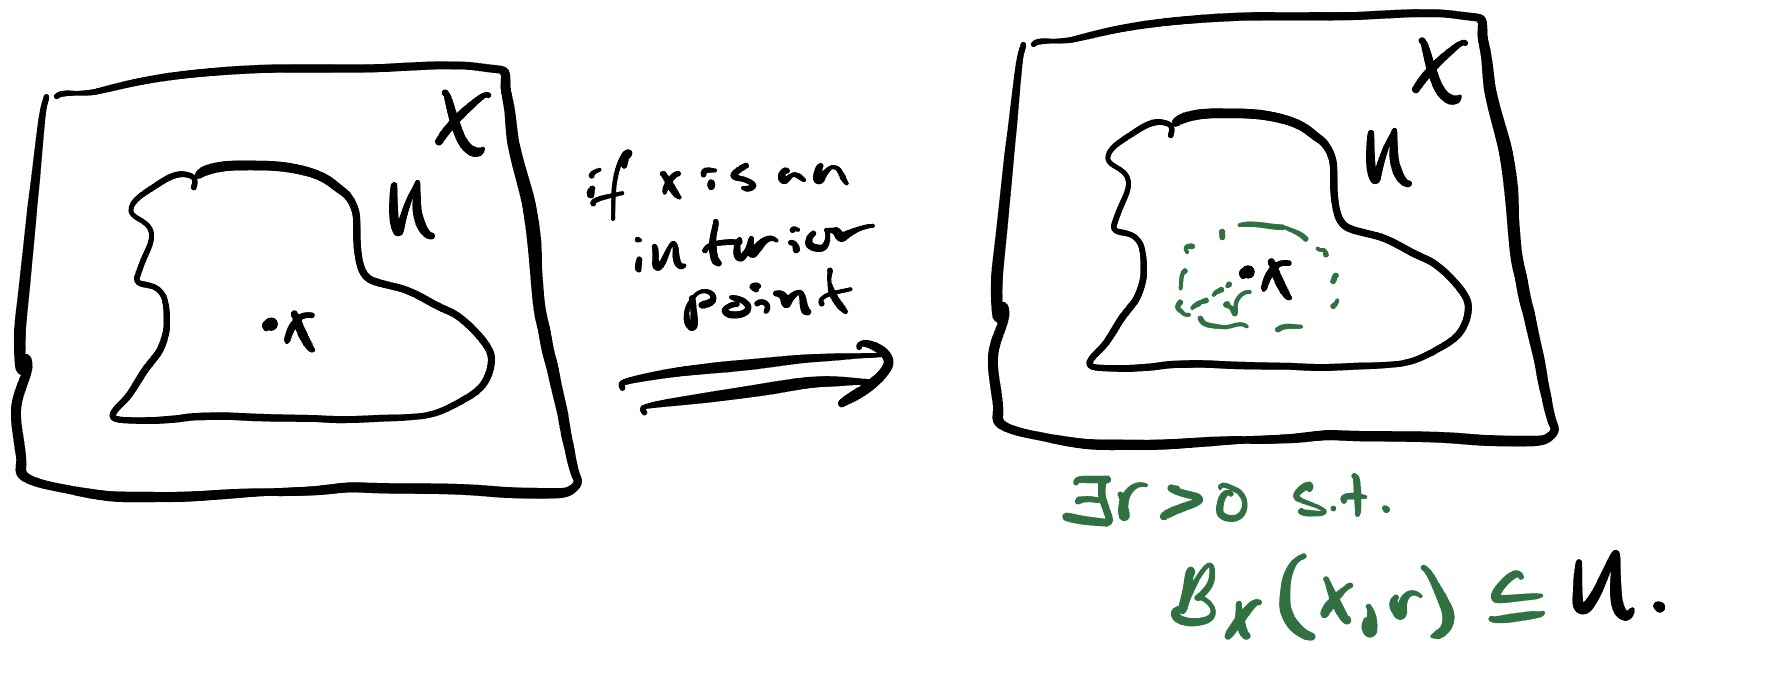
\includegraphics[scale=.17]{m_01.jpg}
\end{figure*}
\end{defi}

Let $(X,d)$ be a metric space. Then suppose we have that $U \subseteq Y \subseteq X$. This implies that $\Int_X (U) \subseteq \Int_Y (U)$ since if we have some $t \in \Int _X (U)$ then there is some $r_t >0$ such that $B_X(t, r_t) \subseteq U$ and as $U \subseteq Y$ then $B_X(t, r_t ) \subseteq Y$ as well, and, unwinding the definitions, we have that $t \in U \subseteq Y$ so $B_Y(t, r_t) \subseteq B_X(t, r_t)$.
\begin{prop} 
Let $(X, d)$ be a metric space; assume $U \subseteq Y \subseteq X$. Then 
\[
\Int _X(U) = \Int _Y (U) \cap \Int _X(Y).
\]
\end{prop}
\begin{proof}
	For the forward inclusion, suppose that $ x \in \Int_X(U)$. Then we have an open ball $B_X(x, \alpha) \subseteq U$. Now our goal here is to find open balls $B_Y (x, \beta) \subseteq U$ and $B_X(x, \gamma) \subseteq Y$. Firstly, we obviously have the latter case already completed for us as $B_X(x, \alpha) \subseteq U \subseteq Y$, by hypothesis. By an identity given earlier, $B_X(x, \alpha) \cap Y = B_Y(x, \alpha)$; yet, as $B_X(x, \alpha )\subseteq U$, then we have that $B_X (x,\alpha) \cap Y \subseteq U$. Thus $B_Y(x, \alpha) \subseteq U$, and we have shows what was necessary. 
	
	For the opposite inclusion, suppose we have $x \in \Int_Y (U)$ and $x \in \Int_X(Y)$. Then there exists a pair of balls around $x$ where $B_X(x, \alpha) \subseteq Y$ and $B_Y(x, \beta) \subseteq U$. We need to find one ball around $x$ for which there is some $\gamma >0$ such that $B_X(x, \gamma) \subseteq U$. For our approach, we will compare these initial radii given by hypothesis. Firstly, if $\alpha = \beta$, then there's nothing really to show since then $B_X(x, \alpha) \subseteq Y$ and $B_ Y (x, \alpha) \subseteq  U$, and so $B_Y(x, \alpha) = B_X(x, \alpha) \cap Y = B_X(x, \alpha)$. Thus $B_X(x, \alpha) = B_Y(x, \alpha) \subseteq U$. Now suppose that $\alpha < \beta$. Then let $t \in B_X(x, \alpha)$, i.e. $t \in X$ and $d(x, t) < \alpha$. But then $d(x,t) < \beta$ as well, and as $B_X(x, \alpha) \subseteq Y$ then $t \in Y$, and so $t \in B_Y(x, \beta) \subseteq U$. Thus $B_X(x, \alpha) \subseteq B_Y(x, \beta) \subseteq U$. Lastly, suppose that $\alpha < \beta$. Recall that, by definition, both the radii are greater than $0$, and so we can find some $\gamma \in \rr$ such that $0 < \gamma < \alpha$. Consider the set $B_X(x, \gamma) = \{ y \in X \colon d(x,y) < \gamma \}$. The clearly if $t \in B_X(x, \gamma)$, then $d(s,t) < \gamma < \beta$. Thus we have that $B_X(x, \gamma) \subseteq  B_X(x, \alpha) \subseteq Y$, and $t \in Y$ as well. This also implies that $t \in B_Y(x, \beta)$ since $t \in Y$ and $d(s,t) < \gamma < \alpha < \beta$, by hypothesis. Thus we have that $B_X(x, \gamma) \subseteq B_Y(x, \beta) \subseteq U$.
\end{proof}

\subsection{ $\S 2.3.$ Open Sets in Metric Spaces}
\begin{defi}
	Let $(X, d)$ be a metric space. A subset $U$ of $X$ is said to be \textbf{open} in $X$ if every point of $U$ is an interior point of $U$ (with respect to $X$); that is, $U = \Int_X( U)$.
\end{defi}
\begin{defi}
We refer to the collection $\mathcal T$ of all open sets of a metric space $(X,d)$ as the \textbf{topology}
of $X$ generated by the metric $d$ (or simply, the topology of $X$, if the metric is clear from context). 	
\end{defi}
\begin{prop}
	Let $(X,d)$ be a metric space. Then $B_X (x,r)$ is open in $X$.
\end{prop}
\begin{proof}
Let $y \in B_X(x,r)$; that is, $y \in X$ and $d(x,y) < r$. We will form a ball around $y$ and show that is open ball in $X$; we only need to choose some `nice' radius for it and the rest follows easily. Let $\delta = r-d(x,y) > 0$. Now what remains to show is that $B_X(y,\delta ) \subseteq B_X(x, r)$. Take $s \in B_X(y, \delta)$. Then $s \in X$ such that $d(y,s) < \delta$. Moreover, $d(x,s) \leq d(s,y) + d(y,x)$, by the triangle inequality of the metric. But as $d(y,s) < \delta = r-d(x,y)$, then $d(x,y)+d(y,s) < r$, and so $d(x,s) <r$; hence $s \in B_X(x,r)$. Thus $B_X(y,\delta ) \subseteq B_X(x,r)$. Therefore if we have some point in $B_X(x,r)$, then we can find a ball around it that's contained in $B_X(x,r)$, i.e. $B_X(x,r)$ is an open set.
\end{proof}
\begin{figure}[h!]
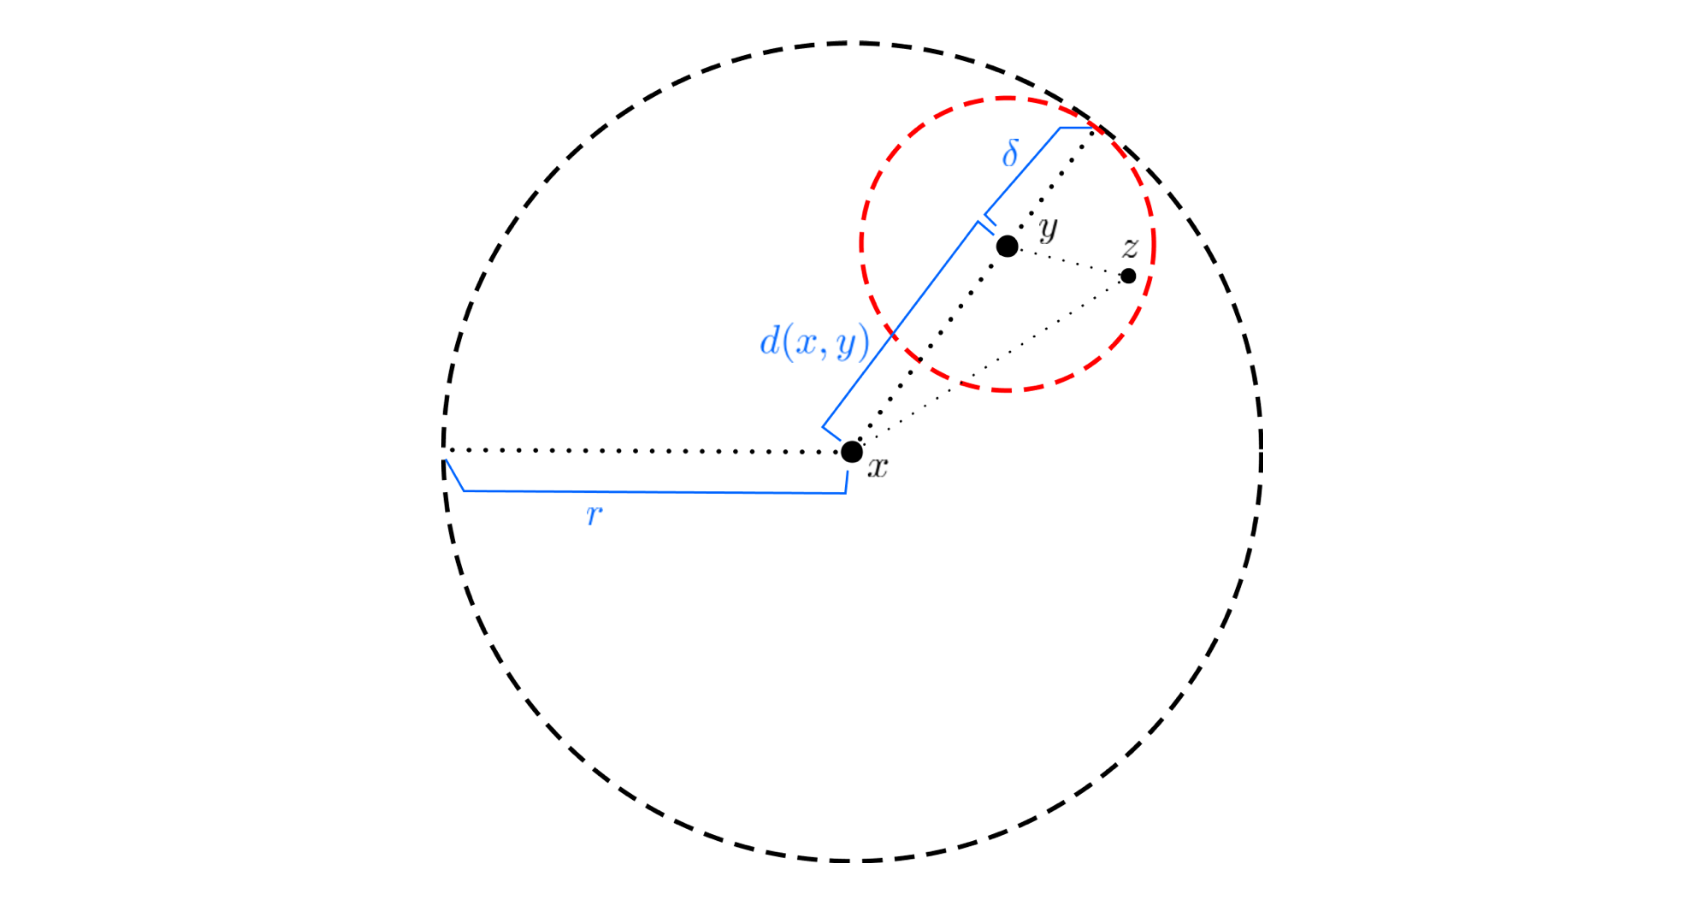
\includegraphics[scale=.5]{m_02.png}
\caption{This how our choice of $\delta = r-d(x,y)$ came about in the preceding proof of Proposition 1.2, and how the triangle inequality to complete the rest of the proof can be easily realized.}
\end{figure}
\begin{rem}
In any metric space $(X,d)$, the empty set is (vacuously) an open set in $X$, and $X$ is (trivially) an open set in $X$. 
\end{rem}
\begin{exercise}[2.7]Let $(X,d)$ be a metric space, and let $U$ be a subset of $X$. Use Proposition [$1.9$] to prove that $\Int _ X (U)$ is open in $X$.
\end{exercise}
\begin{proof}
	We want to show that, essentially, $\Int_X(U) \subseteq \Int_X(\Int_X(U))$. Let $s \in \Int_X(U)$. Then there is some open ball $B_X(s, \alpha) \subseteq U$. We want to find that $s$ has some ball around it such that it is itself contained in $\Int_X(U)$. But as $B_X(s, \alpha)$ is itself open, then for every point $t \in B_X(s, \alpha)$ there is some ball $B_X(t,\beta) \subseteq B_X(s, \alpha) \subseteq U$. Thus if we have some point $t \in B_X(s, \alpha)$, then $t \in \Int_X(U)$, and hence $B_X(s, \alpha) \subseteq \Int_X(U)$. Therefore we have found that if we take some point in the interior of some set, then every point in the corresponding ball is itself an interior point of the original set, i.e. $\Int_X(U) = \Int_X( \Int_X(U))$. 
\end{proof}

\begin{prop}
Let $(X,d)$ be a metric space.
\begin{itemize}
	\item [(i)] Let $\mathfrak U$ be a collection of open sets of $X$. Then the set $\bigcup _{U \in \mathfrak U} U$ is open in $X$.
	\item [(ii)] Let $\{U_1, \ldots, U_n \}$ be a finite collection of open sets of $X$. Then $\bigcap _{i=1}^n U_i$ is an open set of $X$.
\end{itemize}
The \textit{slogan} here is that finite intersections of open sets are open, and finite or infinite unions of open sets are open.	
\end{prop}
\begin{theorem}
	Let $(X,d)$ be a metric space, and let $U$ be a subset of $X$. Then $U$ is open in $X$ if and only if $U$ can be written as a union of open balls $B_X(x,r_x)$ of $X$.
\end{theorem}
\begin{proof}($\Rightarrow$) Assume that $U$ is an open set of $X$. Then for each $x \in X$, there is some $r_x > 0$ such that $B_X(x, r_x) \subseteq U$. Therefore $\bigcup _{x \in U} B_X(x, r_x) \subseteq U$. On the other hand, every $x \in U$ is contained in $B_X(x,r_x)$, so $U$ is contained in the union of these sets. That is, $U = \bigcup _{x \in U} \{x \} \subseteq \bigcup _{x \in U} B_X(x,r_x)$. It follows that $\bigcup _{u \in U} B_X(x, r_x) = U$. ($\Leftarrow$) This direction is easiest as we have that open balls are themselves open, and so if $U$ is itself the union of open balls then it is itself open by the preceding proposition. 
\end{proof}
It is often useful to take \textit{smaller} subsets of $X$ and so it would be of use to consider the open sets of this smaller subset of $X$. Recall that if $(X,d)$ is a metric space and $Y \subseteq X$, then it's obvious that $(Y,d)$ is itself a metric space. We want to consider and clarify the relationships between open sets in $(X,d)$ and the smaller metric space $(Y,d)$. What is essential to remember is that $B_Y(x,r) = B_X(x,r) \cap Y$.
\begin{theorem}
	Let $(X,d)$ be a metric space, and let $U$ and $Y$ be subsets of $X$ such that $U \subseteq Y \subseteq X$. Then $U$ is open in $Y$ if and only if $U = Y \cap V$ for some set $V$ which is open in $X$. 
\end{theorem}
\begin{proof}
	Suppose that $U$ is open in $Y$. Then $U$ is the union of open balls, and so we will write $U = \bigcup _{x \in U} B_Y(x, r_x)  = \bigcup _{x \in U} (B_X(x, r_x) \cap Y) = \bigcup _{x \in U} B_X(x, r_x \cap Y$. We define $V:= \bigcup _{x \in U} B_X(x, r_x)$, which is clearly open in $X$, and so the forward direction follows. Now for the backwards direction suppose we have that $V \subseteq X$ is open and $U = V \cap Y$; we want to show that $U$ is open in $Y$. If $U$ is the empty set, then it is trivially open in $Y$. Thus we assume that $U \neq \varnothing$. Choose $y \in U$. Then we have that $y \in V \cap Y$ and so $y \in V$ implies that there is some $r>0$ such that $B_X(y,r) \subseteq V$. As $B_X(y,r) \subseteq V$ and $y \in Y$, then $B_X(y,r) \cap Y \subseteq  V \cap Y = U$. And so we have that $B_X(y,r) \cap Y = B_Y(y,r)  \subseteq U$ which makes $y$ and interior point of $U$. Thus $y \in \Int _Y(U)$, so $U$ is an open set in $Y$.
\end{proof}

\begin{exercise}[2.8.] Let $(X, d)$ be a metric space. Assume that $U \subseteq Y \subseteq X$, and additionally that $Y$ is open in $X$. Prove that $U$ is open in $Y$ if and only if $U$ is open in $X$. (Note: There at least two possible solutions; one uses Theorem $2.13$, the other uses Exercise $2.5.$)
\end{exercise}
\begin{proof} $(\Rightarrow)$ Suppose that $U$ is open in $Y$. Then $U = Y \cap V$ for some open set $V$ in $X$, but as both $Y$ and $V$ are open in $X$, then $U$ must itself be open in $X$. $(\Leftarrow)$ Suppose that $U$ is open in $X$. Then $U = U \cap Y$ as $U \subseteq Y$, and so as $U$ is open in $X$, then $U = Y \cap V$ is open in $Y$.
\end{proof}

\begin{prop}
Let $(X,d)$ be a metric space, and assume $U \subseteq X$. Then $x \in \Int _X(U)$ if and only if there exists an open subset $V \subseteq X$ such that $x \in V \subseteq U$.
\end{prop}

\begin{proof}($\Rightarrow$) Suppose that $x \in \Int_X(U)$. Then there is some open ball $B_X(x, \alpha)\subseteq U$. But $x \in B_X(x,\alpha)$ as $d(x,x) = 0 < \alpha$, and so, in this case, $V = B_X(x,\alpha)$, which is indeed open. $(\Leftarrow)$ Suppose there exists some open subset $V \subseteq X$ such that $x \in V \subseteq U$. As $V$ is open, then $x \in V = \Int_X(V) \subseteq U$, i.e. $x$ is an interior point and so there is some open ball $B_X(x, \alpha ) \subseteq V \subseteq U$.
\end{proof}
\begin{prop}
Let $(X, d)$ be a metric space. If $V$ is an open set and $V \subseteq U$, then $V \subseteq \Int_X(U)$. Consequently, \[ \Int_X(U) = \bigcup _{V \in \mathcal U} V ;  \; \; \; \;\; \mathcal U = \{S \in \mathcal P(X) \colon S \text{ is open and } S \subseteq U \} \]	
\end{prop}
\begin{proof}
	For the first part, suppose that $V$ is an open set and $V \subseteq U$. Then $\Int_X(V) = V \subseteq U$. By the last proposition, if we take $x \in V \subseteq U$, and $V$ is obviously contained in $X$, then $x \in \Int_X(U)$; thus $V \subseteq \Int_X(U)$. [We could've instead approached this by firstly stating that $\Int_X(V) \subseteq \Int_X(U)$, and as $V$ is open, then this implies that $V = \Int_X(V) \subseteq \Int_X(U)$.]
	
	For the second part of the proposition, suppose that $V \in \mathcal U$. Then we have $V \in \mathcal P(X)$, i.e. $V \subseteq X$, and $V$ is open  with $V \subseteq U$. Thus $V \subseteq \Int_X(U)$. Hence if we chose some $V \in \bigcup _{V \in \mathcal U} V$, then we have the reverse inclusion done. But as $U \subseteq X$, and $\Int_X(U)$ is open in $X$ by Exercise 2.7, then $\Int_X(U) \in \mathcal U$ and thus $\Int_X(U) \subseteq \bigcup_{V \in \mathcal U} V$. Therefore the equality of sets holds true. 
\end{proof}
\subsection{$\S 2.4:$ Equivalent Metrics}

\begin{defi}
Let $X$ be a set, and let $d_1, d_2$ be metrics on $X$. If $d_1$ and $d_2$ generate the same topology, we say that they are \textbf{equivalent metrics}. 	
\end{defi}

\begin{exercise}[2.9]
	Suppose $X$ is a finite, nonempty set and suppose $d$ is a metric on $X$. Let $\mathcal T$ denote the topology generated by $d$. Show that $\mathcal T = \mathcal P(X)$. Conclude that any metric on $X$ is equivalent to the discrete metric. (Hint: To show that $\mathcal T = \mathcal P(X)$, start by proving that $\{x \} = B_{(X,d)} (x, r_x)$ for some sufficiently small $r_x$, for each $x \in X$.)
\end{exercise}
\begin{proof} As $X$ is finite, then it has finitely many subsets. Recall that the topology on a metric space is the collection of all open sets on the metric space $X$ generated by the corresponding metric. Let $E \in \mathcal T$, i.e. $E$ is an open set in $X$. The obviously $E$ must be subset of $X$ by definition of an open set, and so $E \in \mathcal P(X)$. Now suppose that $L \in \mathcal P (X)$, i.e. $L \subseteq X$. Then, as $X$ is finite, then there are finitely many points in $L$; we can enumerate $L$ so that $L = \{p_1, p_2, \ldots, p_n \}$. As $X$ is itself open, then $L \subseteq X = \Int_X(X)$. Then for every point $p_i \in L$, $1 \leq i \leq n$, there is some ball $B_X(p_i, r_i)$ with $r_i > 0$ such that $B_X(p_i, r_i) \subseteq X$. Thus it suffices to show that for any $p_i \in L$, \[ L = \bigcup _{i = 1}^n B_X(p_i, r_i).\] Suppose that $q \in L$. Then there is some open ball $B_X(q, r_q)$ with $r_q > 0$ such that $B_X(q, r_q) \subseteq X$. Thus we see that $q \in \bigcup_{i =1}^n B_X(p_i, r_i)$. Now suppose that $\ell \in \bigcup_{i =1}^n B_X(p_i, r_i)$. Then $\ell \in B_X(p_\alpha, r_\alpha) \subseteq X$ for some $\alpha$. But $B_X(p_\alpha, r_\alpha)$ is constructed by some $p_\alpha \in L$, and $\{p_\alpha \} = B_X(p_\alpha, r_\alpha)$ for some sufficiently small $r_\alpha$. Then $\ell \in \{p_\alpha \}$, i.e. $\ell = p_\alpha \in L$. Thus the equality of sets holds true, and as the right side is a union of open balls in $X$, then $L$ is open in $X$. Hence $L \in \mathcal T$. 
\end{proof}
\begin{exercise}[2.10] Prove that the Euclidean metric and the square metric are equivalent on $\rr^n$.
\end{exercise}
\begin{proof} Recall that the usual Eucidean norm in $\rr^n$ is given taken by comparing two points $p = (a_1, \ldots, a_n)$ and $q = (b_1, \ldots, b_n)$ in $\rr^n$ is given by $d(p,q) = \sqrt{(b_1 - a_1)^2 + \cdots + (b_n - a_n)^2}$. And the square norm is given by $d_u (p,q ) = \max \{ |b_1 - a_1, \ldots, |b_n - a_n | \}$.
	
\end{proof}
\begin{rem}
	In either case that we're working with the Euclidean or square metric on $\rr^n$, we call \textit{this} the standard topology on $\rr^n$.
\end{rem}

\subsection{$\S 3:$ Topological Spaces}
\begin{defi}
Let $X$ be a set. A \textbf{topology} on the set $X$ is a subset $\mathcal T$ of $\mathcal P(X)$, i.e., a collection of subsets of $X$. The collection $\mathcal T$ is required to satisfy the following properties:
	\begin{itemize}
		\item [(1)] $\varnothing, X \in \mathcal T$.
		\item [(2)] $\mathcal T$ is closed under (arbitrary) unions: If $\mathcal U\subseteq \mathcal T$, then $\bigcup _{U \in \mathcal U} U$ is an element of $\mathcal T$.
		\item [(3)] $\mathcal T$ is closed under finite intersections: If $U_1, \ldots, U_n \in \mathcal T$, then $\bigcap _{i=1}^n U_i$ is an element of $\mathcal T$.
	\end{itemize}
	A \textbf{topological space} is a set $X$ together with a topology $\mathcal T$ on $X$, denoted $(X, \mathcal T)$, or simply $X$ when $\mathcal T$ is understood. Elements of $\mathcal T$ are called \textbf{open} subsets of $X$.
\end{defi}

\subsection{$\S 3.2:$ Basis of a Topology}
\begin{defi}
A \textbf{basis} for a topology $\mathcal T$ is a subset $\mathcal B$ of $\mathcal T$ such that every element of $\mathcal T$ can be written as a union of elements of $\mathcal B$. If $\mathcal B$ is a basis for $\mathcal T$, then we refer to $\mathcal T$ as. the topology \textit{generated} by $\mathcal B$.	
\end{defi}
\begin{prop}
Let $X$ be a set, and let $\mathcal B$ be a collection of subsets of $X$, which has the following properties: 
\begin{itemize}
	\item [(1)] Every $x \in X$ is contained in at least one element $B$ of $\mathcal B$.
	\item [(2)] If $B_1, B_2 \in \mathcal B$ and $x \in B_1 \cap B_2$, then there exists a $B_3 \in \mathcal B$ such that $x \in B_3 \subseteq B_1 \cap B_2$.
\end{itemize}
Then the following collection $\mathcal T$ is a topology on $X$: 
\[ \mathcal T = \left \{ U \in \mathcal P(X) \colon U = \bigcup _{B \in \mathcal A} B \text{ for some subcollection } \mathcal A \subseteq \mathcal B \right \}.
\]
and $\mathcal B$ is a basis for $\mathcal T$. On the other hand, if $\mathcal T$ is a topology on $X$ and $\mathcal B$ is a subcollection of $\mathcal T$ such that the preceding equation holds, then $\mathcal B$ must satisfy both properties $(1)$ and $(2)$.
\end{prop}
\begin{exercise} Prove the preceding proposition.
\end{exercise}
\begin{proof} 
For the forward direction, 
\end{proof}

\section{$\S 4$: Analysis on Metric Spaces}
\subsection{Basic Topological Concepts in a Metric Space $\&$ Fundamental Notions}
\subsubsection{Limit Points and Limits of Sequences}
\begin{defi}
Let $(X,d)$ be a metric space. If $U$ is an open set of $X$ containing $x$, we say that $U$ is a \textbf{neighborhood} of $x$ in $X$. The set $B_X(x, \epsilon)$ is called an $\epsilon$\textbf{-neighborhood} of $x$ in $X$.	
\end{defi}
\begin{defi}
Let $(X,d)$ be a metric space; let $E$ be a subset of $X$. A point $x$ is said to be a \textbf{limit point} of $E$ with respect to $X$ if every neighborhood $U$ of $x$ intersects $E \setminus \{x \}$. We will denote the set of all limit points of $E$ with respect to $X$ by $\Lim_X(E)$:
\[ 
\Lim _X(E) = \{ x \in X \colon x \text{ is a limit point of $E$ with respect to $X$ } \}.
\]
A point $x$ is called an \textbf{isolated point} of $E$ with respect to $X$ if $x \in E$ and $x$ is not a limit point of $E$ with respect to $X$. 
\end{defi}
A useful, and easy, observation to make here is that if $x \notin E$, then $E = E \setminus \{x \}$; so that if $x \notin E$, then $x$ is a limit point of $E$ if and only if every neighborhood of $x$ intersects $E$. 

Now we want to look at why it was necessary to actually include the fact that every neighborhood of $x$, in Definition 3.1, had to necessarily be open. Often times you don't need to use that the neighborhood is indeed open to conclude facts about limit points (and the whole collection of limit points).
\begin{prop}
Suppose $(X,d )$ is a metric space; let $E \subseteq X$. Then $x \in \Lim_X(E)$ if and only if for all $\epsilon > 0$, we have that $B_X(x, \epsilon)$ intersects $E \setminus \{x \}$. 	
\end{prop}
\begin{proof}
	For the forward direction, suppose that $x \in \Lim_X(E)$. Then, by definition, for every open neighborhood of $x$ we have that the open neighborhood intersects $E \setminus \{x\}$; in particular, as $x \in B_X(x, \epsilon)$ for any $\epsilon > 0$, then this intersects $E \setminus \{x \}$ since it is indeed an open neighborhood of $x$. For the opposite direction, assume that for all $\epsilon > 0$, we have that $B_X(x, \epsilon)$ intersects $E \setminus \{x \}$, which is to say that $B_X(x, \epsilon) \cap  E \setminus \{x \} \neq \varnothing$. Let $T$ be an open neighborhood of $x$. Then as $T$ is open, then $x$ is an interior point, so $B_X(x, \alpha) \subseteq U$ for some $\alpha > 0$. But we assume that for all $\epsilon > 0$, $B_X(x, \epsilon)$ intersects $E \setminus \{ x\}$, and so $B_X(x, \alpha)$ intersects $E \setminus \{x \}$ as well. Now take $q \in B_X (x, \alpha) \cap E \setminus \{x \}$. Then $q \in B_X(x, \alpha)$ and $ q \in  E \setminus \{x \}$, but $B_X(x, \alpha) \subseteq T$ and so $q \in T \cap E \setminus \{x \}$. Therefore we have that an arbitrary open neighborhood of $x$ intersects $E \setminus \{x \}$. The claim thus follows. 
\end{proof}

\begin{prop}
Let $(X,d)$ be metric space, and $E \subseteq X$. 
\begin{itemize}
	\item[(i)] $\{x \}$ is open in $X$ if and only if there is some $r > 0$ such that $B_X(x,r) = \{ x \}$.
	\item[(ii)] If $\{x \}$ is open in $X$ and $x \in E$, then $x \in \Int_X(E)$, but $x \notin \Lim_X(E)$---$x$ is an isolated point of $E$ with respect to $X$.
	\item[(iii)] If $x \in \Int_X(E)$ and $\{x \}$ is not open in $X$, then $x \in \Lim_X(E)$
\end{itemize}
\end{prop}
\begin{coro}
Given $\rr^n$ the Euclidean metric, and let $E$ be a subset of $\rr^n$. Then $$\Int_{\rr^n} (E) \subseteq \Lim_{\rr^n} (E).$$	
\end{coro}
\begin{prop}
Let $(X,d)$ be a metric space and assume $E \subseteq F \subseteq X$. Then $\Lim _X(E) \subseteq \Lim_X(F)$.
\end{prop}
\begin{proof}
Let $x \in \Lim_X(E)$. Then $x \in X$ such that every open neighborhood $W$ of $x$ intersects with $E \setminus \{ x \}$. So then take $\ell \in W \cap E \setminus \{x \}$. Then $\ell \in W$ and $ \ell \in E \setminus \{x \}$, so then $\ell \in F \setminus \{x \}$. Thus $W$ intersects with $F \setminus \{x \}$, and so $x \in \Lim _X(F)$. Hence the claim follows.
\end{proof}
\end{comment}



\section{Sequences of Functions}
\subsection{Pointwise and Uniform Convergence for Real-Valued Functions.}
Consider the following graph of $f_n (x) = x^n$, this denotes for any given $n \in \zz_{\geq 0}$ we have a corresponding map $f_n : x \mapsto x^n$ from $\rr \to \rr$. In essence, there's a \textit{convergence} to another function for larger and larger $n$:
\begin{figure*}[h!] \label{figure 1}
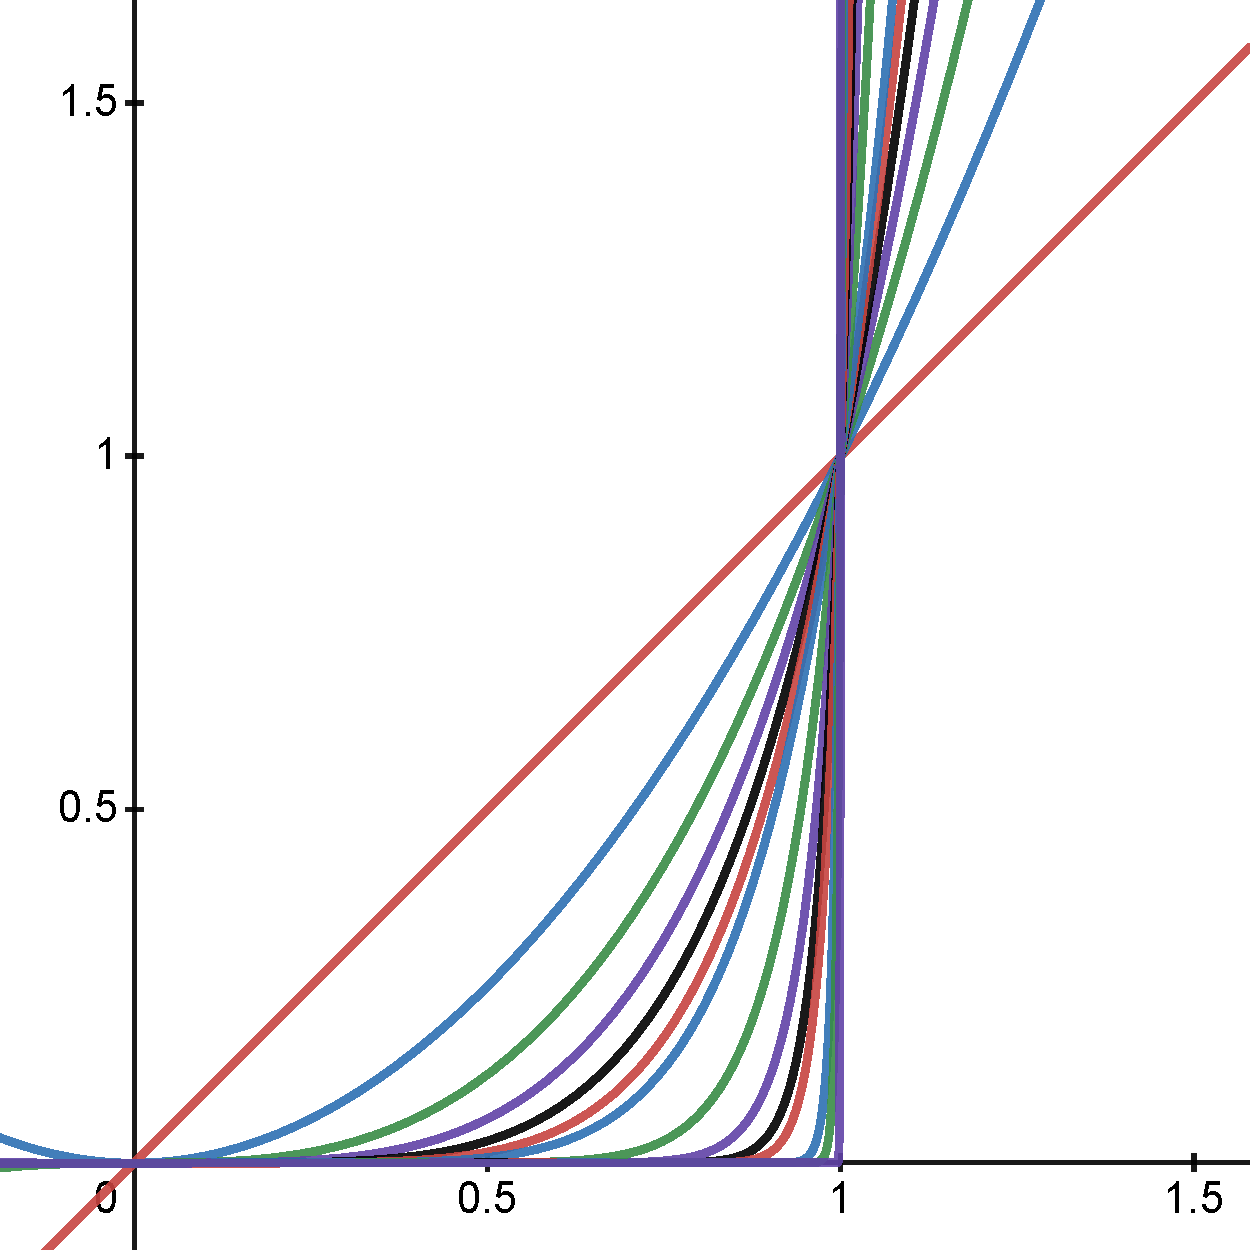
\includegraphics[scale=.3]{images/desmos-graph-3}
\caption{We are particularly focused on the behavior of the first quadrant as this function is not symmetric and the same cannot be said for the the behavior of the second quadrant gets messy.}
\end{figure*}
\begin{defi}
Let $X$ be any set, and let $(f_n)_{n=1}^\infty$ be a sequence of real-valued functions defined on $X$. If for each $x \in E$ the limit $\lim_{n \to \infty} f_n(x)$ exists	, then we can define the (\textbf{pointwise}) \textbf{limit function} by $f(x) = \lim_{n \to \infty} f_n(x)$, for $x \in E$. In this case, we say that $(f_n)$ \textbf{converges pointwise} to $f$ on $E$.
\end{defi}
\begin{ex} \label{ex:1.1}
For $n \in \zz_{\geq 0}$, define $f_n \colon [0,1] \to \rr$ by $f_n(x) = x^n$.	Then for all $x \in [0,1) \subset [0,1]$, we have $f_n(x) =0$ while $f_n(1) = 1$. Hence we form a pointwise function 
\[
f_n(x) = \begin{cases}
	1 & \text{if $x = 1$}\\
	0 & \text{if $x \in [0,1)$}
\end{cases}
\]
\end{ex}
\begin{defi} Let $(X,d_X)$ and $(Y, d_Y)$ be metric spaces; let $f_n\colon X \to Y$ be functions. We say that $(f_n)_{n=1}^\infty$ \textbf{converges uniformly to a function $f \colon X \to Y$} on $E \subset X$ if for every $\epsilon > 0$ there exists an $N \in \nn$ such that for $ n \geq N$ implies $d_Y(f_n(x), f(x)) < \epsilon$ for all $x \in E$. 
\end{defi}
\begin{rem}
This definition is easier to parse when we choose  $Y =\rr^k$; that is, we have a family of functions $f_n \colon X \to \rr^k$ such that we say $(f_n)_{n=1}^\infty$ converges uniformly to a function $f \colon X \to \rr^k$ on $E \subset X$ where for every $\epsilon > 0$ there is an $N\in \nn$ with $n \geq N$ producing $|f_n(x) - f(x)| < \epsilon$ for all $x \in E$.
\end{rem}

\begin{lemma} \label{lem:1.1}
	Assume $f_n \to f$ is pointwise on $E$, and set $$ M_n = \sup_{x \in E} |f_n(x) - f(x)|.$$ Assume additionally that $ M_n < + \infty$ for all $ n \in \nn$. Then $f_n \to f$ uniformly on $E$ if and only if $M_n \to 0$ as $n \to \infty$. 
\end{lemma}
\begin{proof} $(\Rightarrow)$ Let $f_n \to f$ be uniform. We essentially we want to show that $\sup_{x \in E} |f_n(x) - f(x)| < \epsilon$ for any given $\epsilon > 0$ (this is what we mean when we converge to zero, that is, we can pick arbitrarily small $\epsilon$). By uniformity we get some sufficient $n \in \nn$ such that $|f_n(x) - f(x)|<\epsilon/2$ which gives $M_n \leq \epsilon/2<\epsilon$; hence $M_n \to 0$. $(\Leftarrow)$ Let $M_n \to 0$ as $n \to \infty$. Pick $\epsilon >0$ such that for $N \in \nn$ we have $M_n = |\sup_{x \in E} f_n(x) - f(x)| < \epsilon$ and so $|f_n(x) - f(x)| \leq M_n <\epsilon$. Hence $f_n \to f$ uniformly on $E$ as $n \to \infty$. 
\end{proof}
\begin{ex}
If $f_n(x) = x^n$ for all $n \in \nn$ and $x \in \rr$, then $f_n(x) \to 0$, as shown in Example \ref{ex:1.1} (meaning that $f_n(x) \to 0$ for every $x \in [0,1)$ as $ n \to \infty$, i.e. $f_n$ converges to the function $f \colon [0,1) \to \rr$ defined by $f(x) = 0$ for all $x \in [0,1)$, which is denoted by $0$). Now, it turns out that $f_n \to 0$, as defined, converges uniformly on any interval $[0,c]$ for an $0 < c <1$, but $(f_n)$ does not converge uniformly on $[0,1)$.

Let $\epsilon > 0$ and choose $c \in (0,1)$; additionally, write $E = [0,c]$. Then $M_n =\sup_{x \in E} |f_n(x) - f(x)| = \sup_{x \in E} |x^n-0| = \sup_{x \in E} |x^n| =c^n$, and then $M_n \to 0$ as $n \to \infty$ since $0<c<1$. Thus by Lemma \ref{lem:1.1}, we have uniform convergence on $E$. 
\end{ex}
\subsection{Uniform Convergence and the space $B(X)$}
\begin{rem}
For any set $X$, we define $B(X)$ to be the set of (real-valued) functions on $X$ that are bounded. We make this set into a metric space be endowing it with the norm $\|f\|_u = \sup_{x \in X} |f(x)|$ where $f \in X$, which gives a notion of distance defined by for any $f, g \in B(X)$, $d_u(f,g) =\|f-g\| = \sup_{x \in X} |f(x)-g(x)|$---and $B(X)$ also has a vector space structure that \textit{allows} us to do this. In total, $(B(X), \| \cdot \|_u)$ denotes the metric space of (real-valued) functions. We say that two functions $f,g \colon X \to \rr$ are distance $\gamma$ apart in the uniform metric if $\sup_{x \in X} |f(x) -g(x)|\leq \gamma$.
\end{rem}
\begin{prop} \label{prop: 1.1}
Let $(f_n)_{n=1}^\infty$ be a sequence in $B(X)$. Then $f_n \to f$ uniformly on $X$ if and only if \\ $\|f_n-f\|_u \to f$ as $n \to \infty$.	
\end{prop}
\begin{proof} By Lemma \ref{lem:1.1}, $f_n \to f$ uniformly on $X$ if and only if $\sup_{x \in X}|f_n(x) -f(x)|= \|f_n(x)-f (x)\|_u \to 0$ as $n \to \infty$ if and only if $f_n \to f$ in $B(X)$. (Note that this last if and only if statement is what it means for $d_u(f_n,f)$ to tend to zero in $B(X)$.)
\end{proof}
Although the framework of $B(X)$ is nice, it doesn't capture everything that can be said about for a sequence of functions converge uniformly. For example, consider $f_n \colon (0, \infty) \to \rr$ where $f_n(x) = \frac{1}{x} + \frac{1}{n}$ and write $f \colon (0, \infty) \to \rr$ where $f(x) = \frac{1}{x}$. Then $\sup_{x\in (0,\infty)} |f_n(x) - f(x)| = \sup_{x \in (0,\infty)} | \frac{1}{x}+\frac{1}{n}-\frac{1}{x}| = \sup_{x \in (0, \infty)} |\frac{1}{n}| = \frac{1}{n}$ and we know that $1/n \to \infty$ as $n \to \infty$. Hence this sequence is uniform on $(0,\infty)$ and $f_n \to f$. Yet $f_n \notin B((0,\infty))$ for any $n$. But, coming back to Figure \ref{figure 1}, we've just made 'sense' of what we wanted to establish; a notion of convergence to a function, particularly for example we've just established:


\begin{figure*}[h!]
\center{ \frame{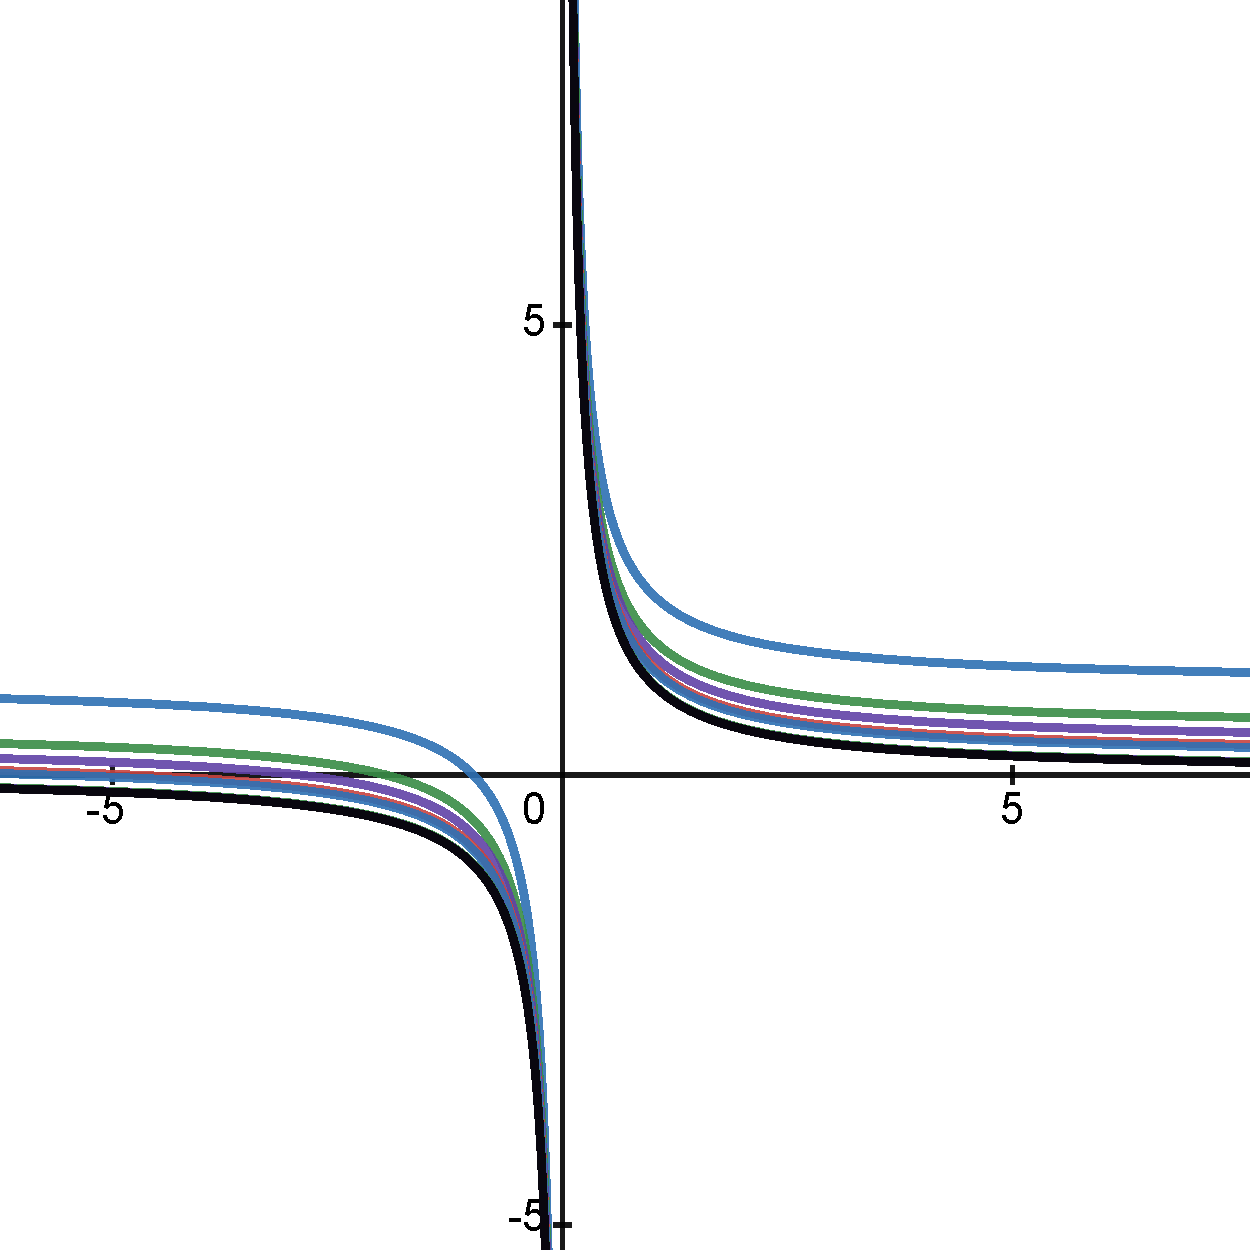
\includegraphics[scale=.3]{images/desmos-graph-4}} }\\
\center{ \frame{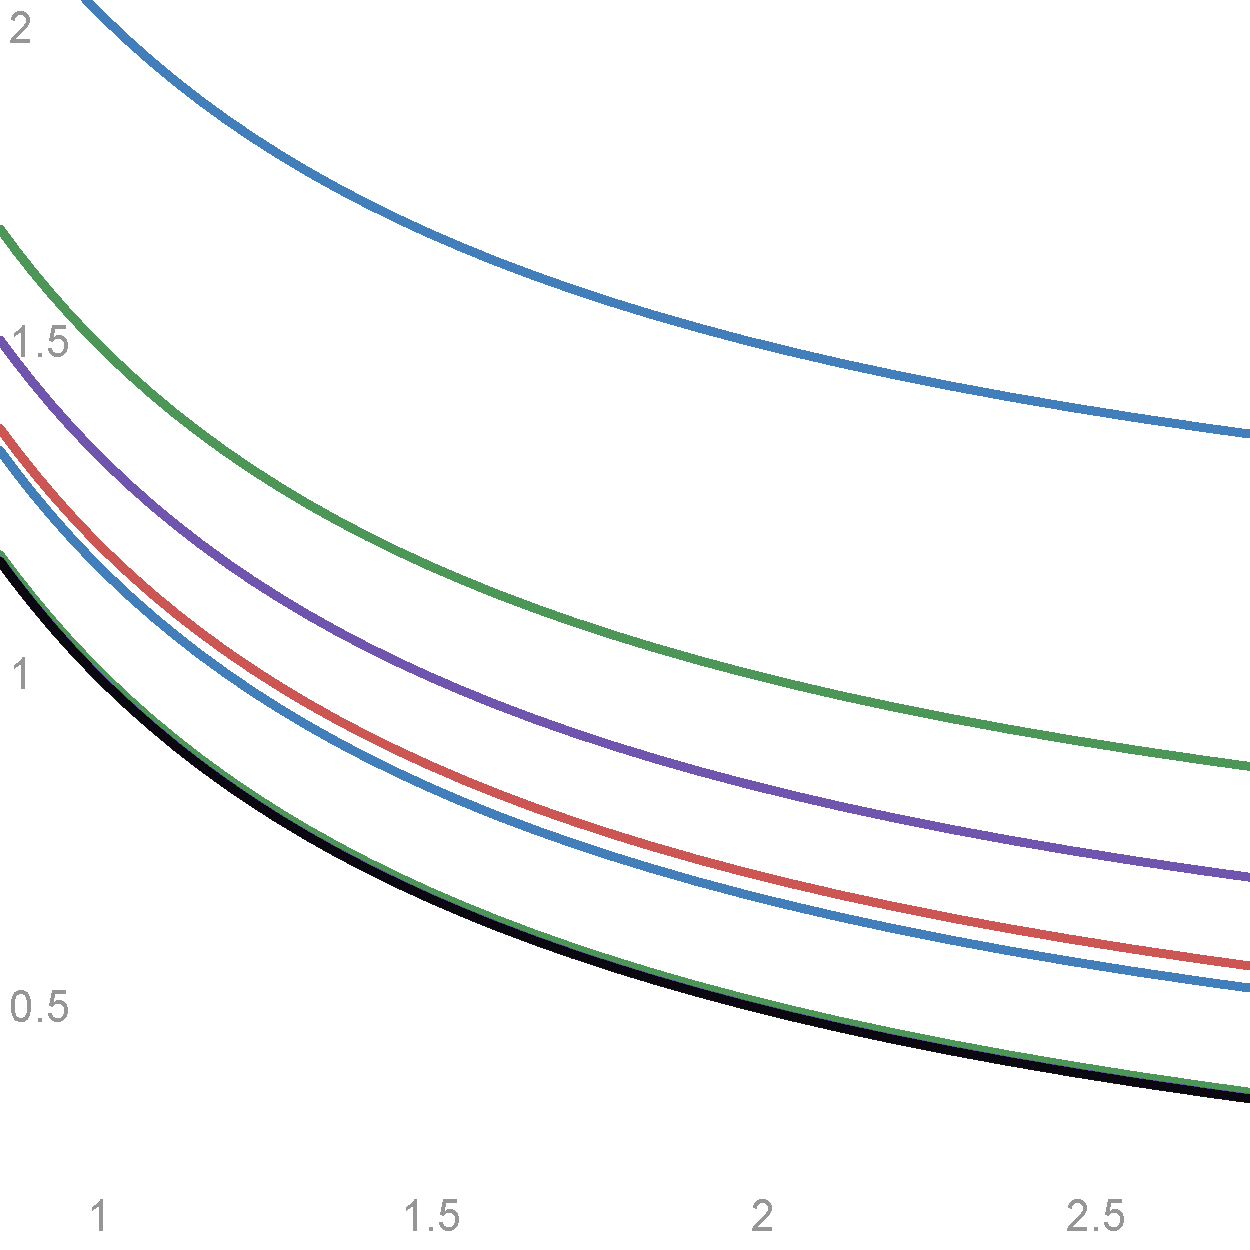
\includegraphics[scale=.23]{images/desmos-graph-5}}} \frame{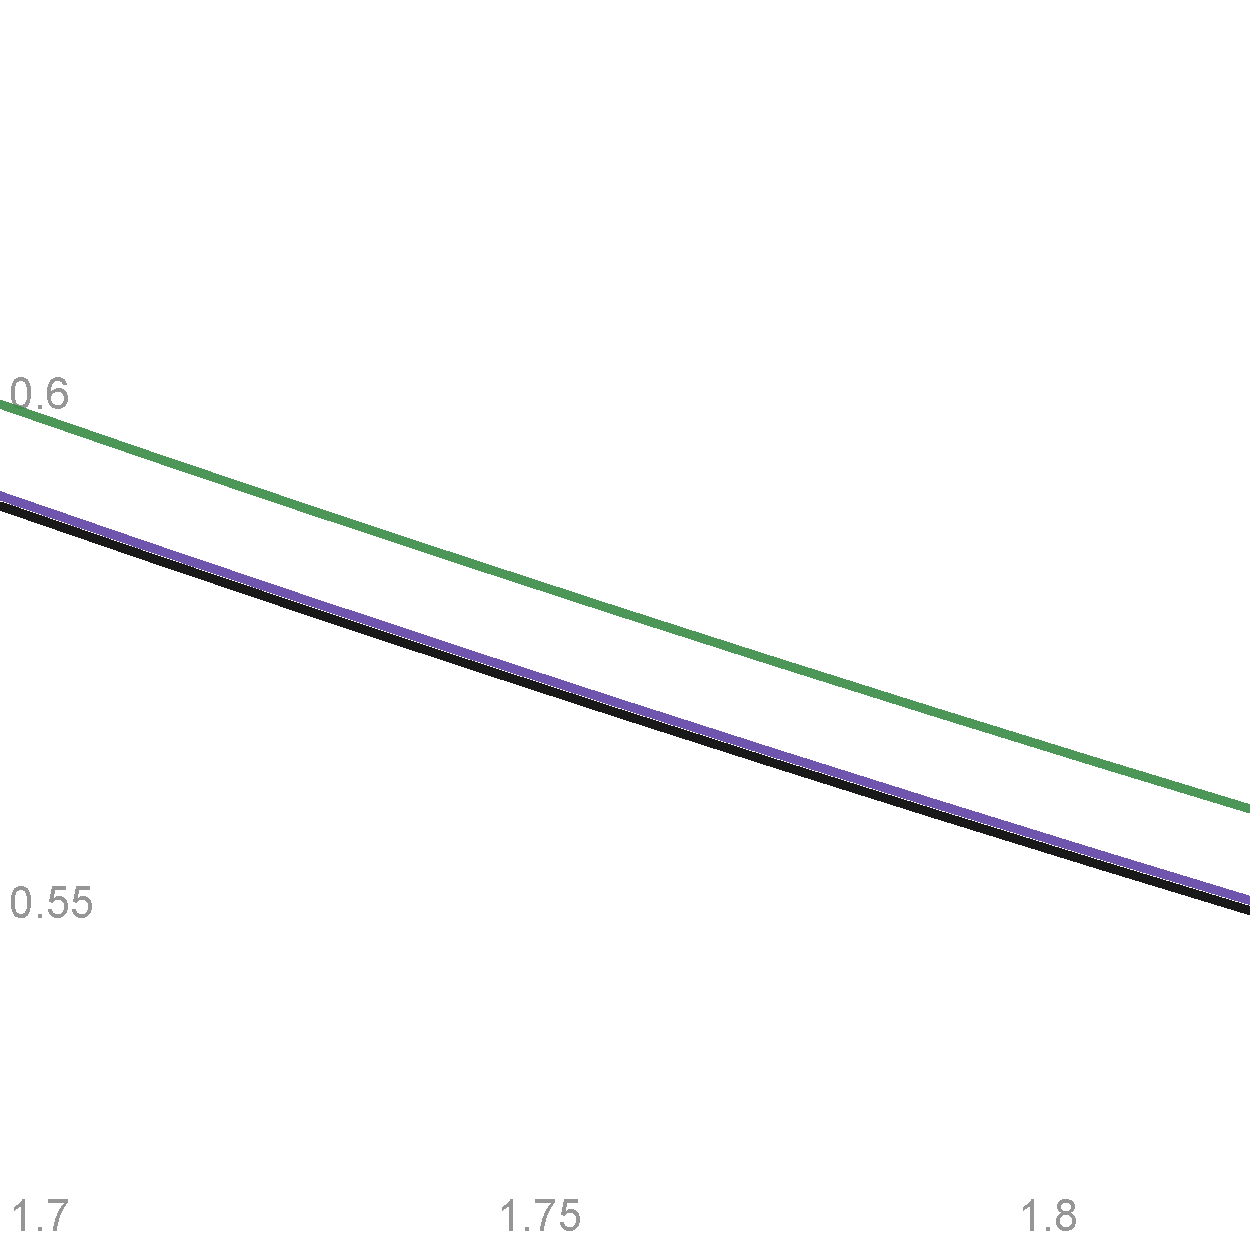
\includegraphics[scale=.23]{images/desmos-graph-6}} 
\caption{$f_n \colon (0, \infty) \to \rr$ defined by $f_n(x) = \frac{1}{x}+\frac{1}{n}$ converges to $f(x) = \frac{1}{x}$ (which is denoted by the pure black line the images).}
\end{figure*}


\begin{tcolorbox}[colback=black!5!white,colframe=black!75!black,title= Exercise $3.1.$]  A collection $\mathcal A$ of real-vlaued functions on a set $E$ is said to be \textbf{uniformly bounded} on $E$ if there exists $M > 0$ such that $|f(x)| \leq M$ for all $x \in E$, for all $f \in \mathcal A$. (So each function is bounded, and the same bound works for all functions in $\mathcal A$.) Let $(f_n)$ be a sequence of bounded functions which converges uniformly to a limit function $f$. Prove that $\{f_n \}_{n=1}^\infty$ is a uniformly bounded subset of $(B(X),d_u)$.
\tcblower 
\begin{proof} As $f_n \to f$, then we may pick $\epsilon = 1$ such that there exists some $N \in \nn$ where $n \geq N$ gives $|f_n - f| < 1$. For each $f_n$, we have that it is bounded by some $M > 0$, i.e. $|f_n| \leq M$. Now write $M = \max \{ M_1, \ldots, M_N\}$. Then $|f_n | \leq |f_n - f|+|f-f_N|+|f_N| < 2+M$. Therefore we have that $ \{ f_n \}_{n=1}^\infty$ is a uniformly bounded subset of $B(X)$.
\end{proof}
\end{tcolorbox}
\begin{tcolorbox}[colback=black!5!white,colframe=black!75!black,title= Exercise $3.2.$] Let $(f_n)_{n=1}^\infty$ and $(g_n)_{n=1}^\infty$ be a sequence of real-valued functions on a set $E$, which converges uniformly on $E$ to limit functions $f$ and $g$, respectively. 
\begin{itemize}
	\item [(a)] Prove that $(f_n+g_n)_{n=1}^\infty$ converges to $f+g$ uniformly on $E$.
	\item [(b)] If each $f_n$ and each $g_n$ is bounded, show that $(f_n g_n)_{n=1}^\infty$ converges uniformly to $fg$ on $E$.
\end{itemize}
\tcblower 
\begin{proof} (a) As $(f_n)_{n=1}^\infty$ and $(g_n)^\infty_{n=1}$ both converge uniformly, we have some $N \in \nn$ and $M \in \nn$ such that for $n \geq N$ and $n \geq M$ we get $ |f_n(x) -f(x)| < \epsilon/2$ and $|g_n(x) - g(x)| < \epsilon/2$, respectively,  for (all) $\epsilon > 0$. Then 
\begin{align*}
|(f_n+g_n)-(f+g)| &= |(f_n-f)+(g_n-g)| \\ &\leq |f_n-f| + |g_n-g| < \frac{\epsilon}{2} + \frac{\epsilon}{2} = \epsilon
\end{align*}
for $ n \geq \max \{M,N\}$. Hence we have $(f_n+g_n)_{n=1}^\infty$ uniformly converging to $f+g$ on $E$.

(b) Suppose that $f_n$ and $g_n$ are bounded; that is, for all $f_n$ and $g_n$, we have $|f_n(x) | \leq M$ and $|g_n(x)| \leq T$ for some $M,P \in \rr$ and all $x \in X$. The idea is two get an $\epsilon/2$ demonstration after applying the triangle inequality many times. As $g_n \to g$, for $\epsilon>0$, there is some $N_1 \in \nn$ such that for $n \geq N_1$ we can write $|g_n-g| < \frac{\epsilon}{2M}$. Additionally, for $\epsilon >0$, there exists some $N_2 \in \nn$ such that $|f_n - f| < (\frac{\epsilon}{2T}-T)$. Then $|f| \leq |f-f_n| + |f_n| = |f_n -f|+|f_n| < (\frac{\epsilon}{2T}) -T+T = \frac{\epsilon}{2T}$. Thus, for $n \geq \max \{N_1, N_2\}$,
\begin{align*}
	|(f_ng_n) -fg| & = |(f_n g_n) - fg + (f_n g- f_ng)| = |(f_ng_n-f_ng)+(f_ng-fg)| \\
	&\leq |f_ng_n-f_ng|+|f_n g-fg| = |f_n (g_n-g)|+|g(f_n-f)| \\
	&= |f_n||g_n-g| + |g||f_n-f| < M \left( \frac{\epsilon}{2M} \right) + (T)\left (\frac{\epsilon}{2T} \right ) = \frac{\epsilon}{2} + \frac{\epsilon}{2} = \epsilon.
\end{align*}

Alternatively, by the previous exercise, we have that $\{f_n \}$ and $\{g_n \}$ is uniformly bounded. Then there exists $M_1, M_2$ such that $|f_n| \leq M_1$ and $|g_n | \leq M_2$; then $ |f_n - g_n| \leq |f_n|+ |g_n| \leq M_1 + M_2$.
\end{proof}
\end{tcolorbox}
\subsection{Uniformly Cauchy Sequences and Completeness of $B(X)$.}
\begin{defi}
A sequence $(f_n)_{n=1}^\infty$ of real-valued functions on a set $X$ is said to be \textbf{uniformly Cauchy} on $E \subset X$ if for every $\epsilon > 0$, there exists $N \in \nn$ such that $m \geq n \geq N$ implies $ |f_m (x) - f_n(x)| < \epsilon$ for all $x \in E$.	
\end{defi}
\begin{prop} \label{prop: 1.2}
If $(f_n)_{n=1}^\infty$ is a Cauchy sequence in $B(X)$, then $(f_n)_{n=1}^\infty$ is uniformly Cauchy on $X$.	
\end{prop}
\begin{proof}
	Let $(f_n)_{n=1}^\infty$ be Cauchy in $B(X)$, i.e. for all $\epsilon > 0$ there is an $N \in \nn$ such that $\|f_n - f_m\|_u < \epsilon$ whenever $m \geq n \geq N$. Then the claim follows when we consider $B(E)$, as the above definition requires it. 
\end{proof}
\begin{theorem}\label{Thm: 1.1.} Let $(f_n)_{n=1}^\infty$ be sequence of real-valued functions on a set $X$. Then $(f_n)_{n=1}^\infty$ converges uniformly $E \subset X$ if and only it is uniformly Cauchy on $E$.
\end{theorem}
\begin{proof} $(\Rightarrow)$ Let $(f_n)_{n=1}^\infty$ converge uniformly on $E$ to $f \colon X \to \rr$. Let $\epsilon > 0$ and pick $N \in \nn$ such that $n \geq N$ gives us $|f_n(x) - f(x)| < \epsilon/2$ for all $x \in E$. Now pick $m \geq n \geq N$, then $ |f_m (x) - f_n(x)| \leq |f_m (x) - f(x) |+ |f_n(x) -f(x)| < \epsilon/2 + \epsilon/2 = \epsilon$. Hence uniformly Cauchy on $E$. $(\Leftarrow)$ Let $(f_n)_{n=1}^\infty$ be uniformly Cauchy on $E$. Then $(f_n(x))_{n=1}^\infty$ is a Cauchy sequence of real numbers for each $x \in E$. Then as $\rr$ is complete, each of the sequences $(f_n(x))_{n=1}^\infty$ converges to some numbers; thus we can have a pointwise limit function $f(x)$. Now pick $\epsilon > 0$ and $N \in \nn$ such that $m \geq n \geq N$ implies $|f_m(x)-f_n(x)| < \epsilon/2$. Suppose $n \geq N$. Then letting $m \to \infty$, then $|f(x)-f_n(x)| = |f_n(x)-f(x) | \leq \epsilon/2 < \epsilon$. Hence $f_n \to f$ converges uniformly. 
\end{proof}
\begin{theorem}
	For any set $X$, the metric space $(B(X), d_u)$ is complete.
\end{theorem}
\begin{proof} We need to show that every Cauchy sequence in $B(X)$ converges. Let $(f_n)_{n=1}^\infty$ be a Cauchy sequence in $B(X)$. By Proposition \ref{prop: 1.2} $(f_n)_{n=1}^\infty$ is uniformly Cauchy and converges uniformly (by Theorem \ref{Thm: 1.1.}) to some $f$ on $E = X \subset X$. It suffices to show that $f \in B(X)$, i.e. we have to show that $|f(x)| \leq M$ for some $M \in \rr_{\geq 0}$. Choose $N \in \nn$ such that $|f_N(x) - f(x) | < 1$ for all $x \in X$ (we can do this by being uniformly Cauchy). As we're working in $B(X)$, every $f_n$ is itself bounded; choose $M > 0$ such that $|f_N(x)| \leq M$. Then $ |f(x)| \leq  |f(x) - f_N(X)| + |f_N(x)| < 1 +M$. Hence $f$ is bounded and therefore $B(X)$ is a complete metric space. 
\end{proof}
\subsection{The Uniform Limit Theorem and completeness of $\text{BC}(X)$ }
\begin{theorem}[Uniform Limit Theorem]
	Let $(f_n)_{n=1}^\infty$ be a sequence of continuous real-valued functions on a metric space $(X,d)$. Assume $f \colon E \to \rr$ is a function such that $f_n \to f$ uniformly on $E \subset X$. Then $f$ is continuous.
\end{theorem}
\begin{proof}
	We proceed via a $\delta$-$\epsilon$ proof; that is, for any $\epsilon > 0$ and $x \in E$, there is a $\delta > 0$ such that $d_X(x,y) < \delta$ implies $|f(x)-f(y)| < \epsilon$. Note that for any $N \in \nn$
	\[
	|f(x)-f(y)| \leq |f(x)-f_N(x)+|f_N(x)-f_N(y)|+|f_N(y)-f(y)|.
	\] As $f_n \to f$ is uniform, then take $|f_N(s)-f(s)| < \epsilon/3$ for any $s \in E$ and this $N \in \nn$. Moreover, pick $\delta > 0$ small enough so that $d(x,y) < \delta$ for $y \in E$ together imply $|f_N(x)-f_N(y)|<\epsilon/3$. Then 
	\begin{align*}
		|f(x)-f(y)| \leq |f(x)-f_N(x)+|f_N(x)-f_N(y)|+|f_N(y)-f(y)| \leq \frac{\epsilon}{3} + \frac{\epsilon}{3}+ \frac{\epsilon}{3} = \epsilon
	\end{align*}
\end{proof}
\begin{defi}
	Let $(X,d)$ be a metric space. The set of all bounded, continuous functions on $X$ is denoted $\text{BC} (X)$.
\end{defi}
\begin{coro}
Let $(X,d)$ be a metric space. The space $(\text{BC}(X), d_u)$ is complete. 	
\end{coro}
\begin{proof}
	It suffices to show that $\text{BC}(X)$ is a closed subset of $B(X)$. Clearly $\text{BC}(X)$ is indeed a subset of $B(X)$. Now let $f$ be a limit point of $\text{BC}(X)$. Then there exists a sequence $(f_n)_{n=1}^\infty$ in $B(X)$ such that $f_n \to f$. By Proposition \ref{prop: 1.1}, $f_n \to f$ is uniform. Then by Uniform Limit Theorem, we have that $f$ is continuous, and hence $f \in \text{BC}(X)$ and $\text{BC}(X)$ is indeed closed. 
\end{proof}
\begin{theorem}[Uniform Limit Theorem, version 2]
\end{theorem}

\section{Working in $\overline{\rr}$ and $\rr$}
\begin{disc} \label{disc: 2.1}
	Recall that $\overline{\rr}$ is defined to be $\overline{\rr} = \rr \cup \{+\infty, -\infty \} $, where the \textit{standard topology} of $\overline{\rr}$ is given by the collection of basis set:  $\mathfrak B_1 = \{ (a, b) \colon a,b \in \rr, a<b \}$, $\mathfrak B_2 = \{ [-\infty, a) \colon a \in \rr \}$, and $\mathfrak B_3 = \{ (b, +\infty] \colon b \in \rr \}$; write $\mathfrak B = \mathfrak B_1 \cup \mathfrak B_2 \cup \mathfrak B_3$. We have the following proposition:
	\begin{prop}
	Let $\mathcal T$ and $\overline{\mathcal T}$ denote the collection of open sets of $\rr$ and and $\overline{\rr}$, respectively. Then $A \in \overline{\mathcal T}$ if and only if $A \cap \rr \in \mathcal T$, i.e. $\mathcal T = \{ A \cap \rr \colon A \in \overline{\mathcal T} \}$.
	\end{prop}
\end{disc}
\subsection{Infinite Limits and Limits at Infinity}
\begin{prop}\
\begin{itemize}
	\item [(a)] If $U$ is a neighborhood of $+\infty$ in $\overline{\rr}$, then there exists an $M \in \rr$ such that $(M, + \infty] \subset U$.
	\item [(b)] If $A \subset \rr$ and $A$ is not bounded above in $\rr$, then $+ \infty$ is a limit point of $A$ with respect to $\overline{\rr}$.
\end{itemize}	
\end{prop}
\begin{proof}(a) Let $U$ be a neighborhood of $+\infty$ in $\overline{\rr}$. As we have a basis described in Discussion \ref{disc: 2.1}, the open set $U$ then contains some $(b, + \infty]$ for some $b \in \rr$ as $U = \cup_{A \in \mathfrak B} A$. Put $M =b$ and we're done.
(b) Let $A \subset \rr$ and let $A$ not be bounded above in $\rr$.
\end{proof}
\begin{prop}
[Infinite Limits and Limits at Infinity] \
\begin{itemize}
	\item [(a)] Let $A$ be subset of $\rr$, let $p \in \rr$ be a limit point of $A$ with respect to $\rr$, and let $f \colon A \to \overline{\rr}$ be a function. Then $$ \lim_{x \to p}f(x) = + \infty$$ if and only if for every $L \in \rr$, there exists $\delta > 0$ such that $0< |x-p|< \delta$ and $x \in A$ together imply that $f(x) > L$.
	\item [(b)] Let $B$ be a subset of $\rr$ that is not bounded above in $\rr$, and let $g \colon B \to \overline{\rr}$ be a function. Let $q$ be a real number. Then $$ \lim_{x \to + \infty} g(x) = q$$ if and only if for every $\epsilon > 0$, there exists $M \in \rr$ such that $x > M$ and $x \in B$ together imply that $ | g(x) -q| < \epsilon$.
	\item [(c)] Let $C$ be a subset of $\rr$ that is not bounded above in $\rr$; let $h \colon C \to \overline{\rr}$ be a function. Then $$ \lim_{x \to + \infty} h(x) = +\infty$$ if and only if for every $N \in \rr$, there exists $P \in \rr$ such that $X>P$ and $x \in C$ together imply $h(x) > N$.
\end{itemize}	
\end{prop}
\begin{proof}(a) Omitted.

(b) Let $\lim_{x \to + \infty} g(x) = q$. The fact that $B$ is not bounded above gives us that $+\infty$ is a limit point of $B$ with respect to $\overline{\rr}$. Then for every neighborhood $V$ of $q$, there is a neighborhood $U$ of $+\infty$ such that $x \in B \cap U \setminus {+\infty}$ implies $f(x) \in V$.
	
\end{proof}

\end{document}